% Heather beetle damage on red grouse count areas: a standalone report for the beetle meeting.
% Build: report/build.sh. Figures and tables: python report/make_figures.py && python report/make_beetle_figures.py
\documentclass[11pt,a4paper]{article}

\newcommand{\reporthead}{Heather beetle damage from satellite imagery}
\newcommand{\reportdate}{October 2026}
% Shared style for the heather management reports (report_v6.tex, beetle_report.tex).
% Each report defines \reporthead and \reportdate before % Shared style for the heather management reports (report_v6.tex, beetle_report.tex).
% Each report defines \reporthead and \reportdate before % Shared style for the heather management reports (report_v6.tex, beetle_report.tex).
% Each report defines \reporthead and \reportdate before \input{style}.
% ---------------------------------------------------------------- fonts and language
\usepackage{amsmath}
\usepackage{fontspec}
\usepackage{unicode-math}
\setmainfont{texgyrepagella}[Extension=.otf,UprightFont=*-regular,BoldFont=*-bold,
  ItalicFont=*-italic,BoldItalicFont=*-bolditalic]
\setsansfont{Helvetica Neue}
\setmathfont{texgyrepagella-math.otf}
\usepackage[british]{babel}
\usepackage{microtype}

% ---------------------------------------------------------------- page
\usepackage[a4paper,top=2.5cm,bottom=2.5cm,left=2.4cm,right=2.4cm,headheight=14pt]{geometry}
\setlength{\parskip}{0.55em}
\setlength{\parindent}{0pt}
\linespread{1.06}

\usepackage{xcolor}
\definecolor{accent}{HTML}{1F4E79}
\definecolor{accentlight}{HTML}{EEF3F9}
\definecolor{muted}{HTML}{5F6B7A}
\definecolor{rulegrey}{HTML}{B8C2CC}

\usepackage{fancyhdr}
\pagestyle{fancy}
\fancyhf{}
\fancyhead[L]{\sffamily\footnotesize\color{muted}\reporthead}
\fancyhead[R]{\sffamily\footnotesize\color{muted}\reportdate}
\fancyfoot[C]{\sffamily\footnotesize\thepage}
\renewcommand{\headrulewidth}{0.4pt}
\renewcommand{\headrule}{\hbox to\headwidth{\color{rulegrey}\leaders\hrule height \headrulewidth\hfill}}
\fancypagestyle{plain}{\fancyhf{}\fancyfoot[C]{\sffamily\footnotesize\thepage}\renewcommand{\headrulewidth}{0pt}}

% ---------------------------------------------------------------- headings and contents
\usepackage{titlesec}
\titleformat{\section}{\sffamily\Large\bfseries\color{accent}}{\thesection}{0.7em}{}
\titleformat{\subsection}{\sffamily\large\bfseries\color{accent}}{\thesubsection}{0.6em}{}
\titleformat{\subsubsection}{\sffamily\normalsize\bfseries}{\thesubsubsection}{0.5em}{}
\titlespacing*{\section}{0pt}{1.8em}{0.6em}
\titlespacing*{\subsection}{0pt}{1.3em}{0.4em}
\titlespacing*{\subsubsection}{0pt}{1.0em}{0.2em}

\usepackage{tocloft}
\renewcommand{\cfttoctitlefont}{\sffamily\Large\bfseries\color{accent}}
\renewcommand{\cftsecfont}{\sffamily\bfseries}
\renewcommand{\cftsecpagefont}{\sffamily\bfseries}
\renewcommand{\cftsecleader}{\cftdotfill{\cftdotsep}}
\setlength{\cftbeforesecskip}{0.2em}
\setlength{\cftbeforetoctitleskip}{0pt}
\setlength{\cftaftertoctitleskip}{0.8em}
\renewcommand{\cftsubsecfont}{\small}
\renewcommand{\cftsubsecpagefont}{\small}
\setlength{\cftbeforesubsecskip}{0pt}
\setcounter{tocdepth}{2}

% ---------------------------------------------------------------- floats, tables, lists
\usepackage{graphicx}
\graphicspath{{figures/}}
\usepackage{booktabs,tabularx,array,threeparttable,makecell}
\renewcommand{\arraystretch}{1.18}
\setlength{\aboverulesep}{0.3ex}
\setlength{\belowrulesep}{0.5ex}
\usepackage{caption}
\captionsetup{font=small,labelfont={bf,sf,color=accent},labelsep=period,justification=justified,
  singlelinecheck=false,skip=6pt}
\captionsetup[table]{position=top}
\usepackage{float}
\usepackage[section]{placeins}
\usepackage{needspace}
\usepackage{enumitem}
\setlist{itemsep=0.25em,topsep=0.3em,parsep=0pt,leftmargin=1.3em}
\newcolumntype{L}{>{\raggedright\arraybackslash}X}

% ---------------------------------------------------------------- boxes and diagrams
\usepackage[most]{tcolorbox}
\newtcolorbox{keybox}[1]{enhanced,breakable,colback=accentlight,colframe=accent,boxrule=0.6pt,arc=1.5pt,
  left=9pt,right=9pt,top=7pt,bottom=7pt,fonttitle=\sffamily\bfseries,coltitle=white,title=#1}
\newtcolorbox{notebox}{enhanced,colback=white,colframe=rulegrey,boxrule=0.5pt,arc=1.5pt,
  left=8pt,right=8pt,top=5pt,bottom=5pt}
\usepackage{tikz}
\usetikzlibrary{positioning,arrows.meta}

% ---------------------------------------------------------------- references and links
\usepackage[round,authoryear]{natbib}
\setlength{\bibsep}{0.35em}
\usepackage{hyperref}
\hypersetup{colorlinks=true,linkcolor=accent,citecolor=accent,urlcolor=accent}

\newcommand{\figref}[1]{Figure~\ref{#1}}
\newcommand{\tabref}[1]{Table~\ref{#1}}
\newcommand{\secref}[1]{Section~\ref{#1}}
\newcommand{\appref}[1]{Appendix~\ref{#1}}

.
% ---------------------------------------------------------------- fonts and language
\usepackage{amsmath}
\usepackage{fontspec}
\usepackage{unicode-math}
\setmainfont{texgyrepagella}[Extension=.otf,UprightFont=*-regular,BoldFont=*-bold,
  ItalicFont=*-italic,BoldItalicFont=*-bolditalic]
\setsansfont{Helvetica Neue}
\setmathfont{texgyrepagella-math.otf}
\usepackage[british]{babel}
\usepackage{microtype}

% ---------------------------------------------------------------- page
\usepackage[a4paper,top=2.5cm,bottom=2.5cm,left=2.4cm,right=2.4cm,headheight=14pt]{geometry}
\setlength{\parskip}{0.55em}
\setlength{\parindent}{0pt}
\linespread{1.06}

\usepackage{xcolor}
\definecolor{accent}{HTML}{1F4E79}
\definecolor{accentlight}{HTML}{EEF3F9}
\definecolor{muted}{HTML}{5F6B7A}
\definecolor{rulegrey}{HTML}{B8C2CC}

\usepackage{fancyhdr}
\pagestyle{fancy}
\fancyhf{}
\fancyhead[L]{\sffamily\footnotesize\color{muted}\reporthead}
\fancyhead[R]{\sffamily\footnotesize\color{muted}\reportdate}
\fancyfoot[C]{\sffamily\footnotesize\thepage}
\renewcommand{\headrulewidth}{0.4pt}
\renewcommand{\headrule}{\hbox to\headwidth{\color{rulegrey}\leaders\hrule height \headrulewidth\hfill}}
\fancypagestyle{plain}{\fancyhf{}\fancyfoot[C]{\sffamily\footnotesize\thepage}\renewcommand{\headrulewidth}{0pt}}

% ---------------------------------------------------------------- headings and contents
\usepackage{titlesec}
\titleformat{\section}{\sffamily\Large\bfseries\color{accent}}{\thesection}{0.7em}{}
\titleformat{\subsection}{\sffamily\large\bfseries\color{accent}}{\thesubsection}{0.6em}{}
\titleformat{\subsubsection}{\sffamily\normalsize\bfseries}{\thesubsubsection}{0.5em}{}
\titlespacing*{\section}{0pt}{1.8em}{0.6em}
\titlespacing*{\subsection}{0pt}{1.3em}{0.4em}
\titlespacing*{\subsubsection}{0pt}{1.0em}{0.2em}

\usepackage{tocloft}
\renewcommand{\cfttoctitlefont}{\sffamily\Large\bfseries\color{accent}}
\renewcommand{\cftsecfont}{\sffamily\bfseries}
\renewcommand{\cftsecpagefont}{\sffamily\bfseries}
\renewcommand{\cftsecleader}{\cftdotfill{\cftdotsep}}
\setlength{\cftbeforesecskip}{0.2em}
\setlength{\cftbeforetoctitleskip}{0pt}
\setlength{\cftaftertoctitleskip}{0.8em}
\renewcommand{\cftsubsecfont}{\small}
\renewcommand{\cftsubsecpagefont}{\small}
\setlength{\cftbeforesubsecskip}{0pt}
\setcounter{tocdepth}{2}

% ---------------------------------------------------------------- floats, tables, lists
\usepackage{graphicx}
\graphicspath{{figures/}}
\usepackage{booktabs,tabularx,array,threeparttable,makecell}
\renewcommand{\arraystretch}{1.18}
\setlength{\aboverulesep}{0.3ex}
\setlength{\belowrulesep}{0.5ex}
\usepackage{caption}
\captionsetup{font=small,labelfont={bf,sf,color=accent},labelsep=period,justification=justified,
  singlelinecheck=false,skip=6pt}
\captionsetup[table]{position=top}
\usepackage{float}
\usepackage[section]{placeins}
\usepackage{needspace}
\usepackage{enumitem}
\setlist{itemsep=0.25em,topsep=0.3em,parsep=0pt,leftmargin=1.3em}
\newcolumntype{L}{>{\raggedright\arraybackslash}X}

% ---------------------------------------------------------------- boxes and diagrams
\usepackage[most]{tcolorbox}
\newtcolorbox{keybox}[1]{enhanced,breakable,colback=accentlight,colframe=accent,boxrule=0.6pt,arc=1.5pt,
  left=9pt,right=9pt,top=7pt,bottom=7pt,fonttitle=\sffamily\bfseries,coltitle=white,title=#1}
\newtcolorbox{notebox}{enhanced,colback=white,colframe=rulegrey,boxrule=0.5pt,arc=1.5pt,
  left=8pt,right=8pt,top=5pt,bottom=5pt}
\usepackage{tikz}
\usetikzlibrary{positioning,arrows.meta}

% ---------------------------------------------------------------- references and links
\usepackage[round,authoryear]{natbib}
\setlength{\bibsep}{0.35em}
\usepackage{hyperref}
\hypersetup{colorlinks=true,linkcolor=accent,citecolor=accent,urlcolor=accent}

\newcommand{\figref}[1]{Figure~\ref{#1}}
\newcommand{\tabref}[1]{Table~\ref{#1}}
\newcommand{\secref}[1]{Section~\ref{#1}}
\newcommand{\appref}[1]{Appendix~\ref{#1}}

.
% ---------------------------------------------------------------- fonts and language
\usepackage{amsmath}
\usepackage{fontspec}
\usepackage{unicode-math}
\setmainfont{texgyrepagella}[Extension=.otf,UprightFont=*-regular,BoldFont=*-bold,
  ItalicFont=*-italic,BoldItalicFont=*-bolditalic]
\setsansfont{Helvetica Neue}
\setmathfont{texgyrepagella-math.otf}
\usepackage[british]{babel}
\usepackage{microtype}

% ---------------------------------------------------------------- page
\usepackage[a4paper,top=2.5cm,bottom=2.5cm,left=2.4cm,right=2.4cm,headheight=14pt]{geometry}
\setlength{\parskip}{0.55em}
\setlength{\parindent}{0pt}
\linespread{1.06}

\usepackage{xcolor}
\definecolor{accent}{HTML}{1F4E79}
\definecolor{accentlight}{HTML}{EEF3F9}
\definecolor{muted}{HTML}{5F6B7A}
\definecolor{rulegrey}{HTML}{B8C2CC}

\usepackage{fancyhdr}
\pagestyle{fancy}
\fancyhf{}
\fancyhead[L]{\sffamily\footnotesize\color{muted}\reporthead}
\fancyhead[R]{\sffamily\footnotesize\color{muted}\reportdate}
\fancyfoot[C]{\sffamily\footnotesize\thepage}
\renewcommand{\headrulewidth}{0.4pt}
\renewcommand{\headrule}{\hbox to\headwidth{\color{rulegrey}\leaders\hrule height \headrulewidth\hfill}}
\fancypagestyle{plain}{\fancyhf{}\fancyfoot[C]{\sffamily\footnotesize\thepage}\renewcommand{\headrulewidth}{0pt}}

% ---------------------------------------------------------------- headings and contents
\usepackage{titlesec}
\titleformat{\section}{\sffamily\Large\bfseries\color{accent}}{\thesection}{0.7em}{}
\titleformat{\subsection}{\sffamily\large\bfseries\color{accent}}{\thesubsection}{0.6em}{}
\titleformat{\subsubsection}{\sffamily\normalsize\bfseries}{\thesubsubsection}{0.5em}{}
\titlespacing*{\section}{0pt}{1.8em}{0.6em}
\titlespacing*{\subsection}{0pt}{1.3em}{0.4em}
\titlespacing*{\subsubsection}{0pt}{1.0em}{0.2em}

\usepackage{tocloft}
\renewcommand{\cfttoctitlefont}{\sffamily\Large\bfseries\color{accent}}
\renewcommand{\cftsecfont}{\sffamily\bfseries}
\renewcommand{\cftsecpagefont}{\sffamily\bfseries}
\renewcommand{\cftsecleader}{\cftdotfill{\cftdotsep}}
\setlength{\cftbeforesecskip}{0.2em}
\setlength{\cftbeforetoctitleskip}{0pt}
\setlength{\cftaftertoctitleskip}{0.8em}
\renewcommand{\cftsubsecfont}{\small}
\renewcommand{\cftsubsecpagefont}{\small}
\setlength{\cftbeforesubsecskip}{0pt}
\setcounter{tocdepth}{2}

% ---------------------------------------------------------------- floats, tables, lists
\usepackage{graphicx}
\graphicspath{{figures/}}
\usepackage{booktabs,tabularx,array,threeparttable,makecell}
\renewcommand{\arraystretch}{1.18}
\setlength{\aboverulesep}{0.3ex}
\setlength{\belowrulesep}{0.5ex}
\usepackage{caption}
\captionsetup{font=small,labelfont={bf,sf,color=accent},labelsep=period,justification=justified,
  singlelinecheck=false,skip=6pt}
\captionsetup[table]{position=top}
\usepackage{float}
\usepackage[section]{placeins}
\usepackage{needspace}
\usepackage{enumitem}
\setlist{itemsep=0.25em,topsep=0.3em,parsep=0pt,leftmargin=1.3em}
\newcolumntype{L}{>{\raggedright\arraybackslash}X}

% ---------------------------------------------------------------- boxes and diagrams
\usepackage[most]{tcolorbox}
\newtcolorbox{keybox}[1]{enhanced,breakable,colback=accentlight,colframe=accent,boxrule=0.6pt,arc=1.5pt,
  left=9pt,right=9pt,top=7pt,bottom=7pt,fonttitle=\sffamily\bfseries,coltitle=white,title=#1}
\newtcolorbox{notebox}{enhanced,colback=white,colframe=rulegrey,boxrule=0.5pt,arc=1.5pt,
  left=8pt,right=8pt,top=5pt,bottom=5pt}
\usepackage{tikz}
\usetikzlibrary{positioning,arrows.meta}

% ---------------------------------------------------------------- references and links
\usepackage[round,authoryear]{natbib}
\setlength{\bibsep}{0.35em}
\usepackage{hyperref}
\hypersetup{colorlinks=true,linkcolor=accent,citecolor=accent,urlcolor=accent}

\newcommand{\figref}[1]{Figure~\ref{#1}}
\newcommand{\tabref}[1]{Table~\ref{#1}}
\newcommand{\secref}[1]{Section~\ref{#1}}
\newcommand{\appref}[1]{Appendix~\ref{#1}}


\hypersetup{pdftitle={Heather beetle damage on red grouse count areas, summer 2025},
  pdfauthor={Sabeeth, Game and Wildlife Conservation Trust}}

\begin{document}

% ================================================================ title page
\begin{titlepage}
\newgeometry{top=2.4cm,bottom=2.2cm,left=2.4cm,right=2.4cm}
\raggedright
{\color{accent}\rule{\linewidth}{1.6pt}}\par\vspace{0.9cm}
{\fontsize{27}{34}\selectfont\bfseries\color{accent}Heather beetle damage\\ on red grouse count areas,\\ summer 2025\par}
\vspace{0.45cm}
{\Large\itshape\color{muted}Measuring damage from Sentinel-2 satellite imagery, tested against the July 2025 survey\par}
\vspace{0.7cm}
{\sffamily\large Sabeeth\par}
{\sffamily\normalsize\color{muted}Game \& Wildlife Conservation Trust \enspace\textbullet\enspace October 2026\par}
\vspace{0.6cm}
{\color{rulegrey}\rule{\linewidth}{0.5pt}}\par
\vspace{0.7cm}
\begin{tcolorbox}[enhanced,colback=accentlight,colframe=accentlight,arc=1.5pt,left=11pt,right=11pt,top=9pt,bottom=9pt]
{\sffamily\bfseries\color{accent}Abstract}\par\vspace{0.3em}
\small
An outbreak of heather beetle damaged heather across red grouse moors in northern England in 2025, and a field survey in July 2025 scored the proportion of 23 red grouse count areas damaged. We tested whether Sentinel-2 satellite imagery can measure the same damage. Beetle-killed heather browns in the summer it is attacked and greys as the dead leaves drop, so we measured two changes: the drop in the Normalised Burn Ratio from summer 2024 to summer 2025 (browning), and the loss of colour from early to late summer 2025 (greying), each beyond the change across all count areas, with burnt and cut ground left out. The share of each count area showing either change is a rule-based estimate that uses nothing from the survey. We then trained gradient boosting on pixels labelled automatically from the survey, undamaged count areas against heavily damaged ones, and averaged the two estimates. Tested only on moors the model had not seen, the final estimate is within 0.1 of the survey on 15 of 22 count areas and within 0.2 on 19, with a typical difference of 0.10 and a rank agreement of 0.88. Predicting each count area from its regional average gives 0.17. The red-edge bands carry much of the signal, and the result holds up to checks for data leakage. The method also gives estimates for the five Eggleston count areas the survey did not score. Field photos, a second survey year and damage records from 2024 are the next steps.
\end{tcolorbox}
\vspace{0.5cm}
{\small\color{muted}This report uses the count area polygon boundaries digitised by Eleanor and the July 2025 heather beetle damage survey. It is a companion to the report on heather burning and cutting on the same count areas (version 2, October 2026).\par}
\restoregeometry
\end{titlepage}

% ================================================================ contents
\newgeometry{top=1.8cm,bottom=1.9cm,left=2.4cm,right=2.4cm}
\pagenumbering{roman}
\thispagestyle{plain}
\tableofcontents
\clearpage
\restoregeometry
\pagenumbering{arabic}

% ================================================================ key findings
\section*{Key findings}
\addcontentsline{toc}{section}{Key findings}

\begin{keybox}{Main results}
\begin{itemize}
\item \textbf{Sentinel-2 can see heather beetle damage.} Count areas the survey scored as more damaged browned and greyed more over summer 2025 (rank correlations of 0.56 and 0.63 with the survey) (\secref{sec:signals}).
\item \textbf{The final estimate is close to the survey:} within 0.1 on 15 of 22 count areas and within 0.2 on 19, with a typical difference of 0.10 and a rank agreement of 0.88. Predicting from the regional average, with no satellite data, gives 0.17 (\secref{sec:agreement}).
\item \textbf{No hand labelling was needed.} The model's training labels came automatically from the survey: pixels in count areas scored 0 as healthy, in count areas scored 0.5 or more as damaged.
\item \textbf{The two steps complement each other.} The rule-based estimate captures the full range of damage; gradient boosting learns what is not damage, such as the colour change across the whole bog at Moor House, Trout Beck (\secref{sec:learns}).
\item \textbf{The red-edge bands carry much of the signal.} Four of the ten measures the model relies on most are red-edge, which respond to the loss of chlorophyll.
\item \textbf{The result holds up to leakage checks.} Choosing the model inside each test fold gives 0.105 against 0.098, and hiding a whole region from training still gives 0.07 for the combined estimate on that region (\secref{sec:trust}).
\item \textbf{Five Eggleston count areas the survey did not score} have estimates of 0.15 to 0.27, except Neamour at 0.55 (\secref{sec:byarea}).
\item \textbf{Damage is not clearly visible a year later.} Summer 2026 against summer 2024 barely follows the survey (rank correlation $-0.13$).
\end{itemize}
\end{keybox}

\begin{keybox}{For discussion}
\begin{itemize}
\item \textbf{How were the survey scores estimated?} Walked transects, viewpoints or a whole-area judgement affect how closely any satellite estimate can match.
\item \textbf{Field photos} from July 2025, ideally with locations, especially for Wemmergill, South Side (survey 0.6, satellite 0.24), Moor House, Trout Beck (0, satellite 0.30) and Edmundbyers, Waskerley (0, satellite 0.20).
\item \textbf{Damage scores from 2024,} if any were recorded, would show when the outbreak started and test the method on a second year.
\item \textbf{Neamour, Eggleston} reads 0.55 but was not surveyed. Is that consistent with what managers saw?
\end{itemize}
\end{keybox}

\clearpage
% ================================================================ 1 introduction
\section{Introduction}\label{sec:intro}

\subsection{Heather beetle}

Heather beetle feeds on heather. In outbreak years it can kill the foliage over large areas: attacked heather turns red-brown in the summer of the attack, then grey as the dead leaves drop. Heavy damage was reported across the red grouse moors of northern England in 2025. It matters for grouse, which depend on heather for food and cover, and for moor management: PW reports that managers burnt and cut beetle-killed heather to promote recovery, and the heather burning and cutting report finds 2024/25 the most heavily managed season in nine years.

\subsection{The July 2025 survey}

A survey in July 2025 estimated, by eye, the proportion of each red grouse count area damaged by heather beetle. It scored 23 count areas in tenths, from 0 to 0.8 (\tabref{tab:survey}). Damage was heaviest on the North York Moors and in the southern Dales. In the northern Dales most count areas were undamaged, but a few were heavily damaged.

\begin{table}[htbp]
\centering
\caption{The July 2025 survey by GWCT region.}\label{tab:survey}
\small
\begin{tabular}{lrrrr}
\toprule
Region & \makecell[r]{Count areas\\scored} & \makecell[r]{Mean\\damage} & Range & \makecell[r]{Scored 0\\(no damage)} \\
\midrule
North York Moors & 5 & 0.62 & 0.5 to 0.8 & 0 \\
Southern Dales and Peak & 3 & 0.50 & 0.2 to 0.7 & 0 \\
Northern Dales & 15 & 0.15 & 0.0 to 0.6 & 8 \\
\midrule
\textbf{All} & 23 & 0.30 & 0.0 to 0.8 & 8 \\
\bottomrule
\end{tabular}

\end{table}

\subsection{Aims}

\begin{enumerate}
\item Find out whether Sentinel-2 imagery shows heather beetle damage, and which changes carry it.
\item Estimate the proportion of each count area damaged, and measure how close the estimate is to the survey.
\item Test how far the estimate can be trusted on moors it has not seen.
\item Look at how the damage relates to heather burning and cutting.
\end{enumerate}

\subsection{What was done}

\begin{enumerate}
\item \textbf{Measured change in four Sentinel-2 images} for every count area: summer 2024 (before the outbreak), early and late summer 2025, and summer 2026, with burnt and cut ground left out.
\item \textbf{Built a rule-based estimate} from browning and greying, with nothing fitted to the survey.
\item \textbf{Trained gradient boosting} on pixels labelled automatically from the survey, after comparing six models, and averaged it with the rule.
\item \textbf{Tested every estimate on moors left out of training,} and checked for data leakage with a nested model choice, whole-region hold-outs and bootstrap intervals.
\item \textbf{Examined the imagery} where satellite and survey agree and disagree most.
\item \textbf{Estimated the five count areas the survey did not score.}
\end{enumerate}

\FloatBarrier
% ================================================================ 2 data
\section{Data}\label{sec:data}

\subsection{Count areas}

The count areas are the 28 red grouse count areas (4,273~ha, 16 moors) digitised by Eleanor (GWCT), the same as in the burning and cutting report. The survey scored 23 of them. Grinton, Long Gill had too few clear images in summer 2024 to be estimated, which leaves 22 count areas for comparison. Five Eggleston count areas were not surveyed; they are estimated but cannot be checked.

\subsection{Satellite imagery}

Sentinel-2 Level-2A surface reflectance, with cloud, cloud shadow and snow masked, was combined into four images, each the median of all clear scenes in its window (\tabref{tab:windows}). A count area needs at least three clear scenes per pixel in each window.

\begin{table}[htbp]
\centering
\caption{The four images.}\label{tab:windows}
\small
\begin{tabular}{lll}
\toprule
Image & Window & Role \\
\midrule
Summer 2024 & 1 July to 30 September 2024 & Before the main damage \\
Early summer 2025 & 16 April to 30 June 2025 & Before the late-summer damage \\
Late summer 2025 & 1 July to 30 September 2025 & Damage visible; matches the July survey \\
Summer 2026 & 1 July to 30 September 2026 & A year later \\
\bottomrule
\end{tabular}
\end{table}

\subsection{Burnt and cut ground}

Burning and cutting also remove heather and would look like damage. Ground detected as burnt or cut in 2024/25 or 2025/26 by the heather management analysis, plus a 20~m margin around it, is left out of every estimate.

\FloatBarrier
% ================================================================ 3 methods
\section{Methods}\label{sec:methods}

\subsection{What damage looks like from space}

\begin{itemize}
\item \textbf{Browning.} Dead and dying heather reflects less near-infrared and more short-wave infrared, so the Normalised Burn Ratio, $\mathrm{NBR} = (\mathrm{NIR}-\mathrm{SWIR2})/(\mathrm{NIR}+\mathrm{SWIR2})$, falls.
\item \textbf{Greying.} As the dead leaves drop, the canopy loses its colour. Colour saturation, the spread between the brightest and darkest of the blue, green and red bands relative to the brightest, falls towards zero for a grey surface.
\item \textbf{Red edge.} Three Sentinel-2 bands (B5, B6, B7, 20~m) sit on the steep rise in reflectance between red and near-infrared, which depends on chlorophyll. They respond early to stressed and dying leaves.
\end{itemize}

Summer 2025 was dry and the whole area browned to some degree, so every change is measured \emph{beyond} its median across all count areas.

\begin{figure}[htbp]
\centering
\begin{tikzpicture}[
  node distance=0.4cm and 0.5cm,
  box/.style={draw=accent,fill=accentlight,rounded corners=2pt,align=center,font=\sffamily\footnotesize,
              minimum height=1.35cm,text width=3.05cm,inner sep=4pt},
  key/.style={draw=accent,fill=accent,text=white,rounded corners=2pt,align=center,font=\sffamily\footnotesize\bfseries,
              minimum height=1.35cm,text width=3.05cm,inner sep=4pt},
  arr/.style={-{Stealth[length=2mm]},color=accent,thick}]
\node[box] (img) {Four Sentinel-2 images, 2024 to 2026; burnt and cut ground left out};
\node[box,right=of img] (rule) {\textbf{Step 1:} share of pixels that browned or greyed beyond the moor-wide change};
\node[box,right=of rule] (lab) {Pixels labelled from the survey: 0 healthy, 0.5 or more damaged};
\node[box,right=of lab] (gb) {\textbf{Step 2:} gradient boosting on 45 changes per pixel};
\node[key,below=1.05cm of gb] (fin) {Final estimate: average of the two steps};
\node[box,left=of fin] (test) {Tested on moors left out of training};
\node[box,left=of test] (leak) {Leakage checks: nested choice, region hold-out, bootstrap};
\node[box,left=of leak] (img2) {Imagery where satellite and survey differ};
\draw[arr] (img) -- (rule); \draw[arr] (rule) -- (lab); \draw[arr] (lab) -- (gb);
\draw[arr] (gb) -- (fin);
\draw[arr,dashed] (fin) -- (test); \draw[arr,dashed] (test) -- (leak); \draw[arr,dashed] (leak) -- (img2);
\end{tikzpicture}
\caption{How the estimate is made (solid arrows) and tested (dashed arrows).}\label{fig:flow}
\end{figure}

\subsection{Step 1: a rule-based estimate}

A pixel is \textbf{flagged} as damaged if, beyond the moor-wide change, its NBR fell by more than 0.10 from summer 2024 to summer 2025 (browning), or its colour saturation fell by more than 0.05 from early to late summer 2025 (greying). The rule-based estimate is the \textbf{share of each count area flagged}. The cut-offs were set from the imagery, not fitted to the survey.

\subsection{Step 2: gradient boosting with labels from the survey}

About 280 pixels were sampled in each count area. Each pixel is described by 45 changes: all ten Sentinel-2 bands and five indices (NBR, NDVI, NDMI, colour saturation and brightness), each for three comparisons (summer 2025 against 2024, late against early summer 2025, and summer 2026 against 2024). Pixels in count areas the survey scored 0 were labelled healthy and pixels in count areas scored 0.5 or more were labelled damaged; count areas in between were not used as labels. No labels were drawn by hand.

Gradient boosting \citep{friedman2001} builds its prediction from many small decision trees, each correcting the errors of those before it. For each count area, the mean probability of damage across its pixels is converted to a proportion with a straight line fitted on the training count areas. Six models were compared (\appref{app:models}); classic gradient boosting did best and is used here.

\subsection{Final estimate and testing}

The \textbf{final estimate is the average of the two steps.} Every estimate is made by a model that has not seen the moor being predicted (leave-one-moor-out; \citealp{roberts2017}). Agreement with the survey is summarised as:
\begin{itemize}
\item \textbf{typical difference:} the mean absolute difference between estimate and survey;
\item \textbf{within 0.1} and \textbf{within 0.2:} the number of count areas that close to the survey;
\item \textbf{rank agreement:} Spearman's rank correlation, which measures whether the estimate puts the count areas in the same order as the survey.
\end{itemize}
As a benchmark with no satellite data, each count area is predicted as the average damage of the other moors in its region. The formulae are in \appref{app:formulae}.

\FloatBarrier
% ================================================================ 4 results
\section{Results}\label{sec:results}

\subsection{Which changes follow the damage}\label{sec:signals}

\begin{table}[htbp]
\centering
\caption{Rank correlation between each change, as the median over the count area, and the surveyed damage. 22 count areas. A negative value means count areas with more damage lost more.}\label{tab:signals}
\small
\begin{tabular}{lr}
\toprule
Measure (median over the count area) & \makecell[r]{Rank correlation\\with the survey} \\
\midrule
Browning: NBR, summer 2025 against summer 2024 & $-$0.56 \\
Greying: colour saturation, late against early summer 2025 & $-$0.63 \\
Colour saturation, summer 2025 against summer 2024 & $-$0.64 \\
Greenness: NDVI, summer 2025 against summer 2024 & $-$0.40 \\
A year later: NBR, summer 2026 against summer 2024 & $-$0.13 \\
\textbf{Share of count area flagged (rule-based estimate)} & +0.81 \\
\bottomrule
\end{tabular}

\end{table}

Both browning and greying follow the survey (\tabref{tab:signals}): count areas with more damage lost more NBR between summers 2024 and 2025 and more colour over summer 2025. Greenness (NDVI) follows it less closely. The change from 2024 to 2026 barely follows the survey at all: by summer 2026 the heather had partly recovered, or the damaged heather had been burnt or cut and is left out. Combining browning and greying into the share of each count area flagged gives a rank correlation of 0.81.

\subsection{Agreement with the survey}\label{sec:agreement}

\begin{figure}[htbp]
\centering
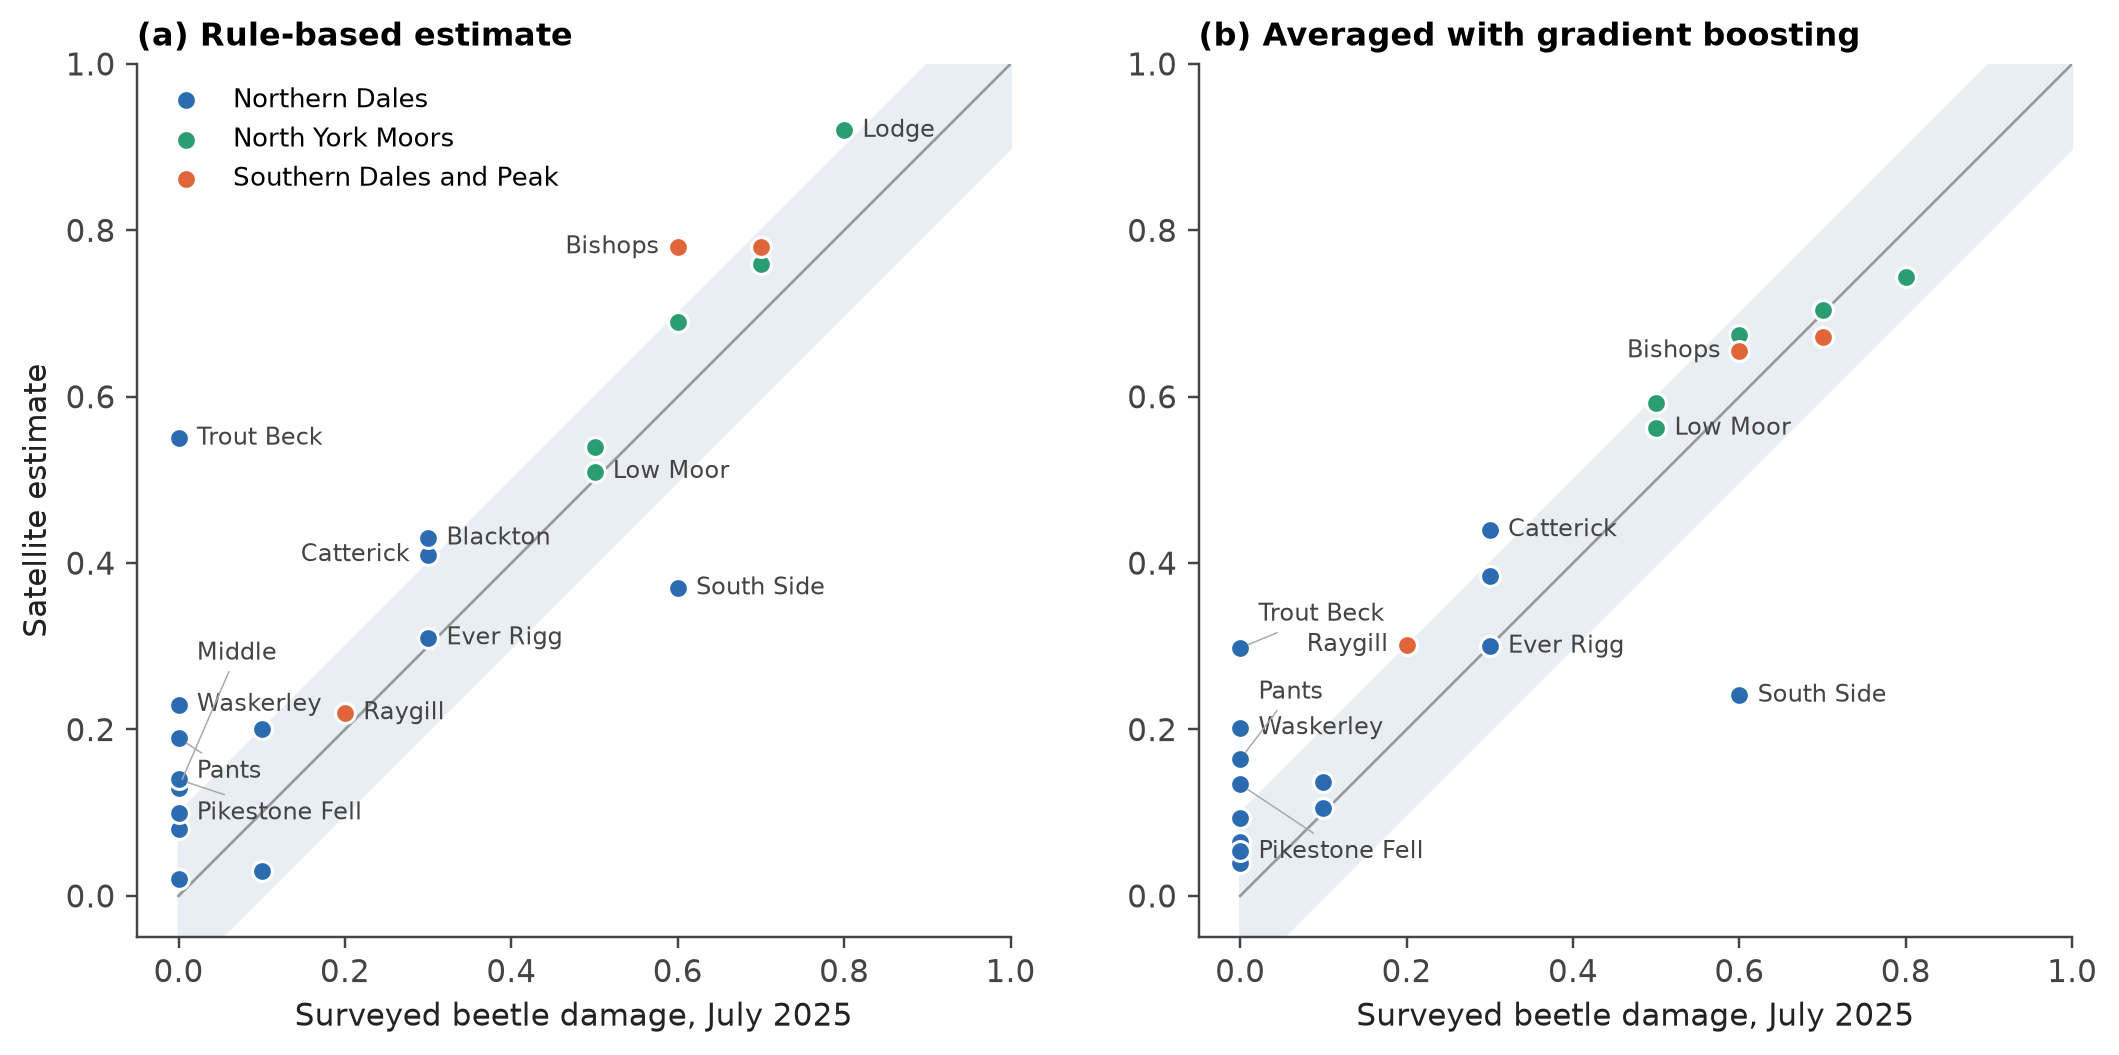
\includegraphics[width=\linewidth]{fig_beetle_gb.png}
\caption{Satellite estimates against the July 2025 survey: (a) the rule-based estimate; (b) the final estimate, the rule averaged with gradient boosting. Each moor is predicted without its own data. The shaded band is within 0.1 of the survey. Count areas more than 0.1 from the survey, or discussed in the text, are labelled.}\label{fig:scatter}
\end{figure}

\begin{table}[htbp]
\centering
\caption{From the first attempt to the final estimate. 22 count areas, each moor predicted without its own data.}\label{tab:progress}
\small
\begin{tabular}{>{\raggedright\arraybackslash}p{7.2cm}rrrr}
\toprule
Estimate & \makecell[r]{Typical\\difference} & \makecell[r]{Within\\0.1} & \makecell[r]{Within\\0.2} & \makecell[r]{Rank\\agreement} \\
\midrule
Browning only & 0.27 & 2 & 7 & 0.60 \\
Browning or greying, beyond the moor-wide change & 0.13 & 11 & 19 & 0.83 \\
+ 20 m margin round burns and cuts (rule-based estimate) & 0.12 & 12 & 19 & 0.81 \\
\textbf{+ averaged with gradient boosting (final estimate)} & \textbf{0.10} & \textbf{15} & \textbf{19} & \textbf{0.88} \\
\midrule
Gradient boosting alone & 0.12 & 10 & 20 & 0.79 \\
Region average, no satellite data & 0.17 & 4 & 16 & 0.38 \\
\bottomrule
\end{tabular}

\end{table}

The final estimate is \textbf{within 0.1 of the survey on 15 of 22 count areas and within 0.2 on 19}, with a typical difference of 0.10 (\figref{fig:scatter}, \tabref{tab:progress}). It ranks the count areas almost as the survey does (0.88), against 0.38 for the regional average.

Each step added something (\figref{fig:progress}). Browning alone, measured against no reference, read too high everywhere because the whole area browned in the dry summer; measuring change beyond the moor-wide median and adding greying halved the error. Leaving out a 20~m margin round burns and cuts removed fresh burn edges counted as damage. Averaging with gradient boosting brought three more count areas within 0.1 of the survey.

\begin{figure}[htbp]
\centering
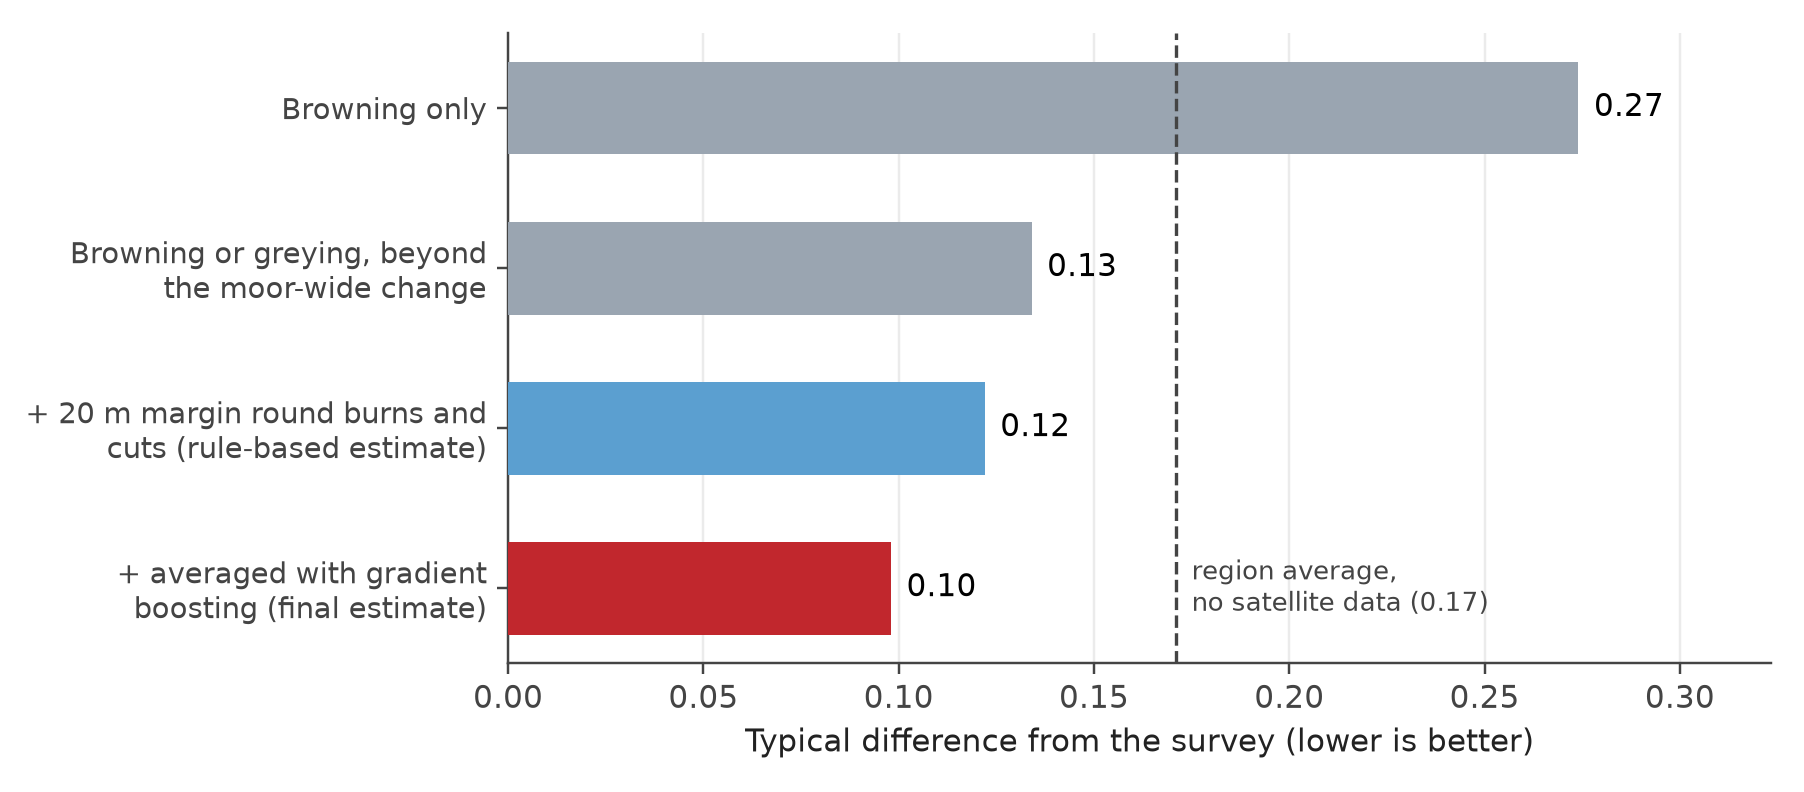
\includegraphics[width=0.84\linewidth]{beetle_fig_progress.png}
\caption{Typical difference from the survey at each step. The dashed line is the regional average, with no satellite data.}\label{fig:progress}
\end{figure}

\subsection{Count area by count area}\label{sec:byarea}

\begin{figure}[htbp]
\centering
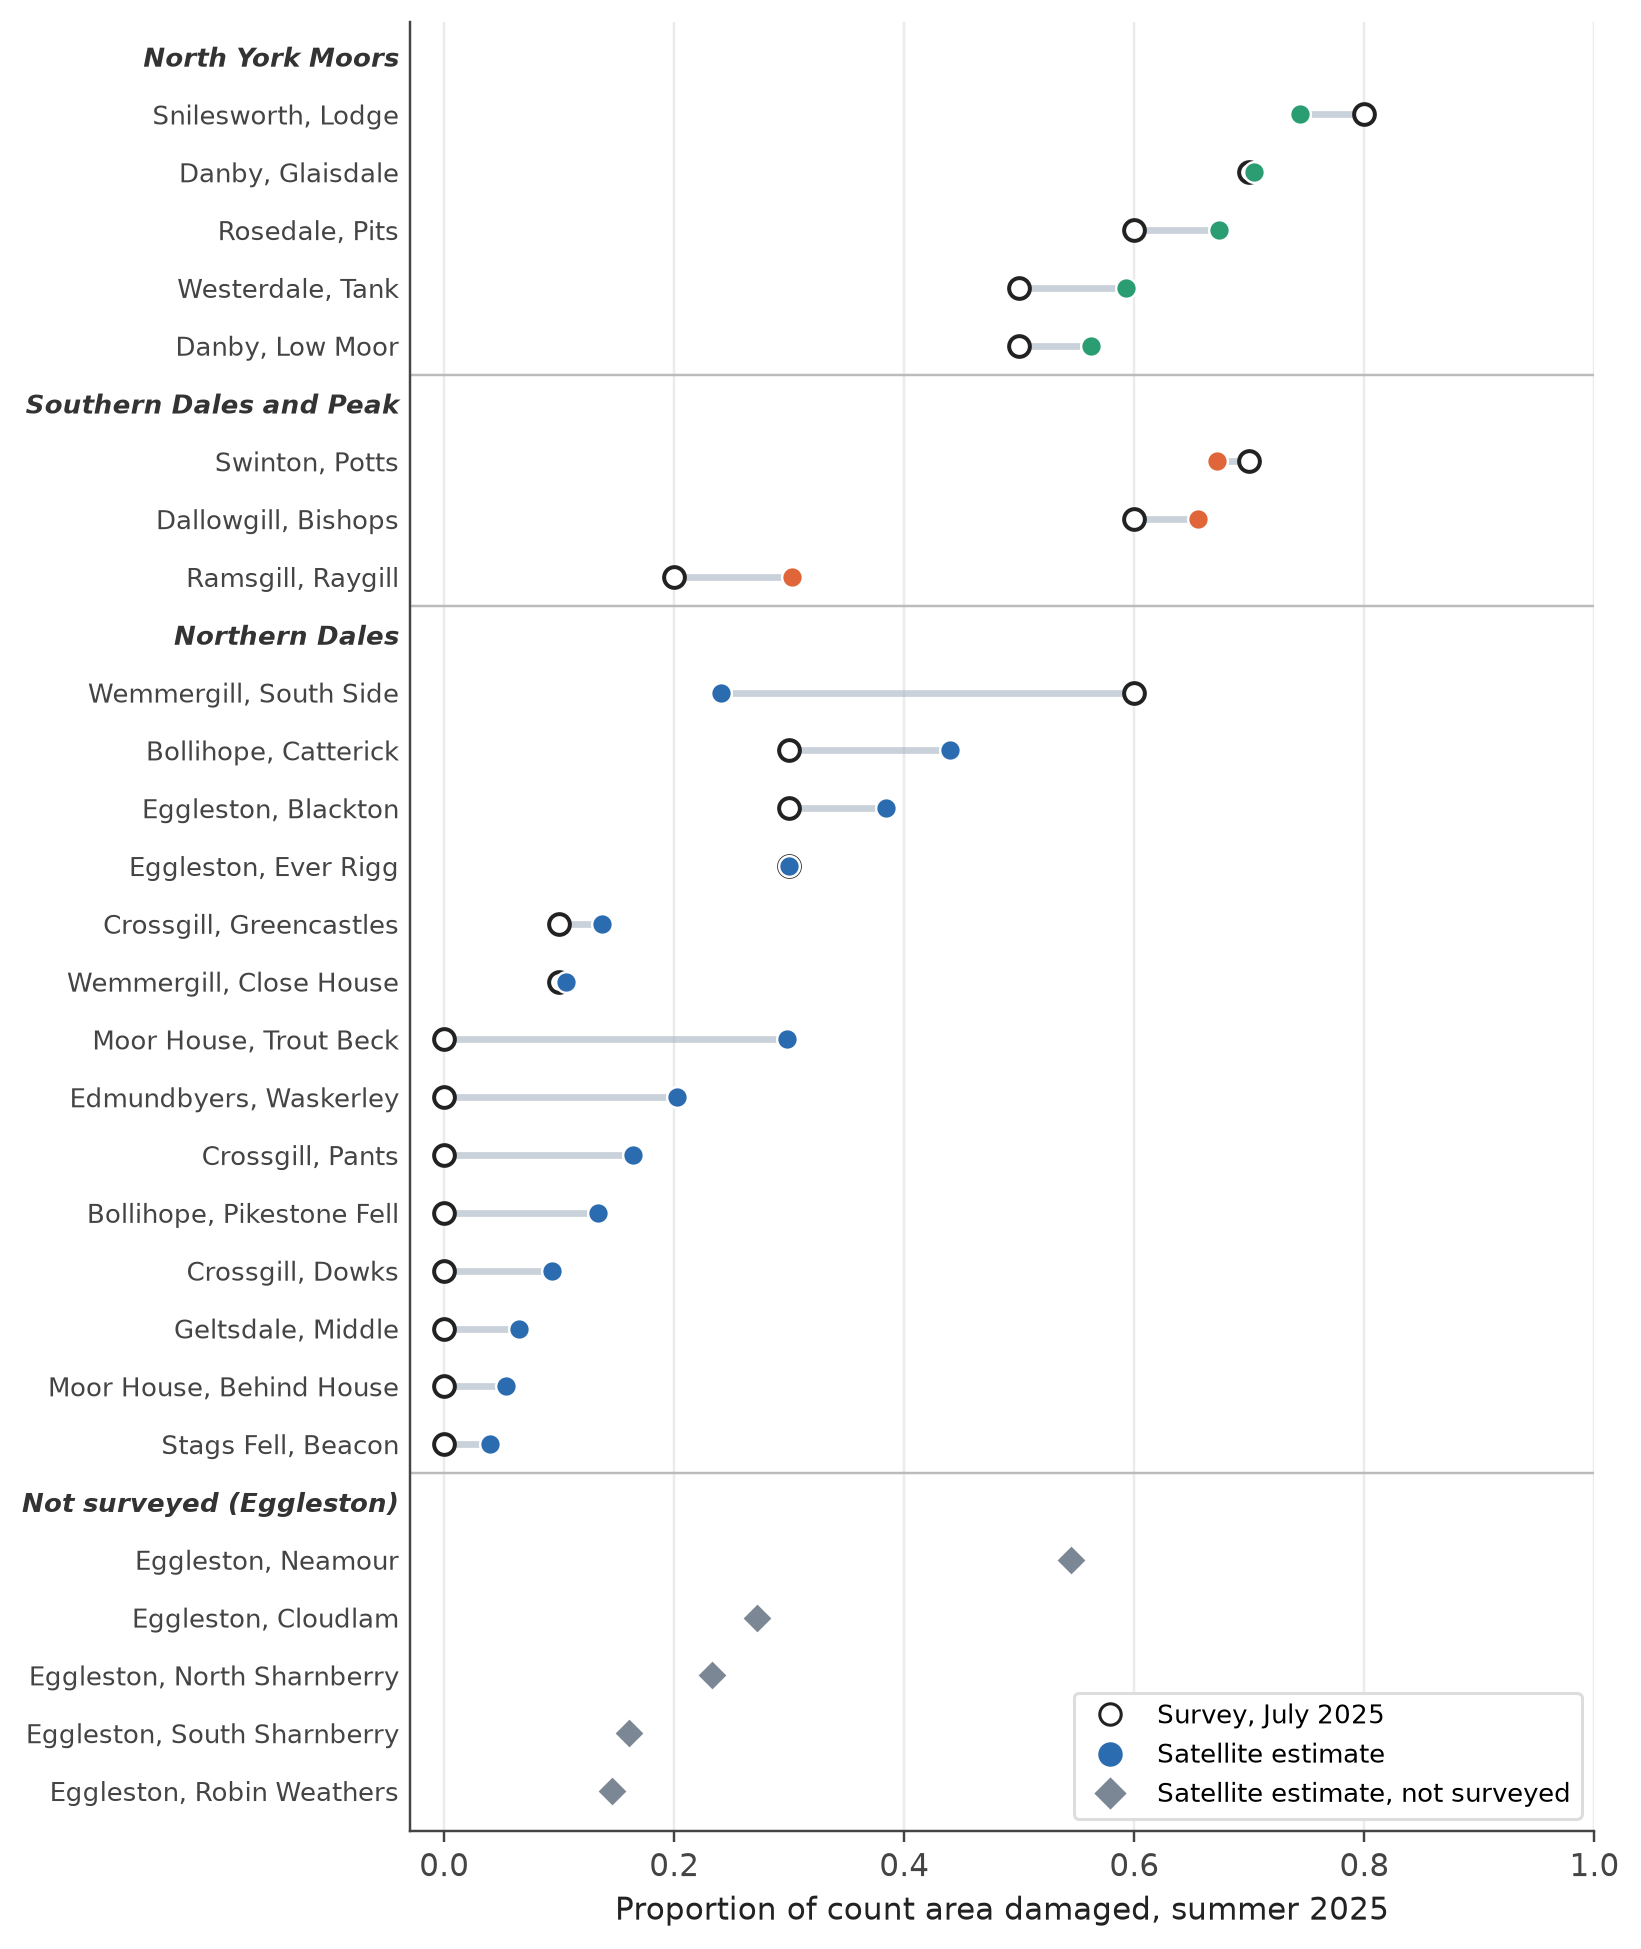
\includegraphics[width=0.86\linewidth]{beetle_fig_by_area.png}
\caption{Surveyed damage (open circles) and the final satellite estimate (filled circles, coloured by region) for each count area, and estimates for the five Eggleston count areas the survey did not score (diamonds).}\label{fig:byarea}
\end{figure}

On the North York Moors and in the southern Dales, where damage was heavy, all eight count areas are within 0.11 of the survey (\figref{fig:byarea}; values in \appref{app:areas}). In the northern Dales most count areas were undamaged, and the estimate reads slightly high there: on average about 0.11 above the survey where it found little or no damage (0 to 0.1). Three count areas differ by more than 0.2: Moor House, Trout Beck (\secref{sec:learns}), Edmundbyers, Waskerley (just over, round its burns) and Wemmergill, South Side, where the satellite finds less damage than the survey (\secref{sec:imagery}).

\textbf{Count areas not surveyed.} The five Eggleston count areas the survey did not score read 0.15 to 0.27, similar to Blackton and Ever Rigg (surveyed 0.3), except \textbf{Neamour at 0.55}. Both steps read Neamour high (rule 0.70, gradient boosting 0.39). It is worth checking with the estate.

\subsection{What gradient boosting learns}\label{sec:learns}

\begin{figure}[htbp]
\centering
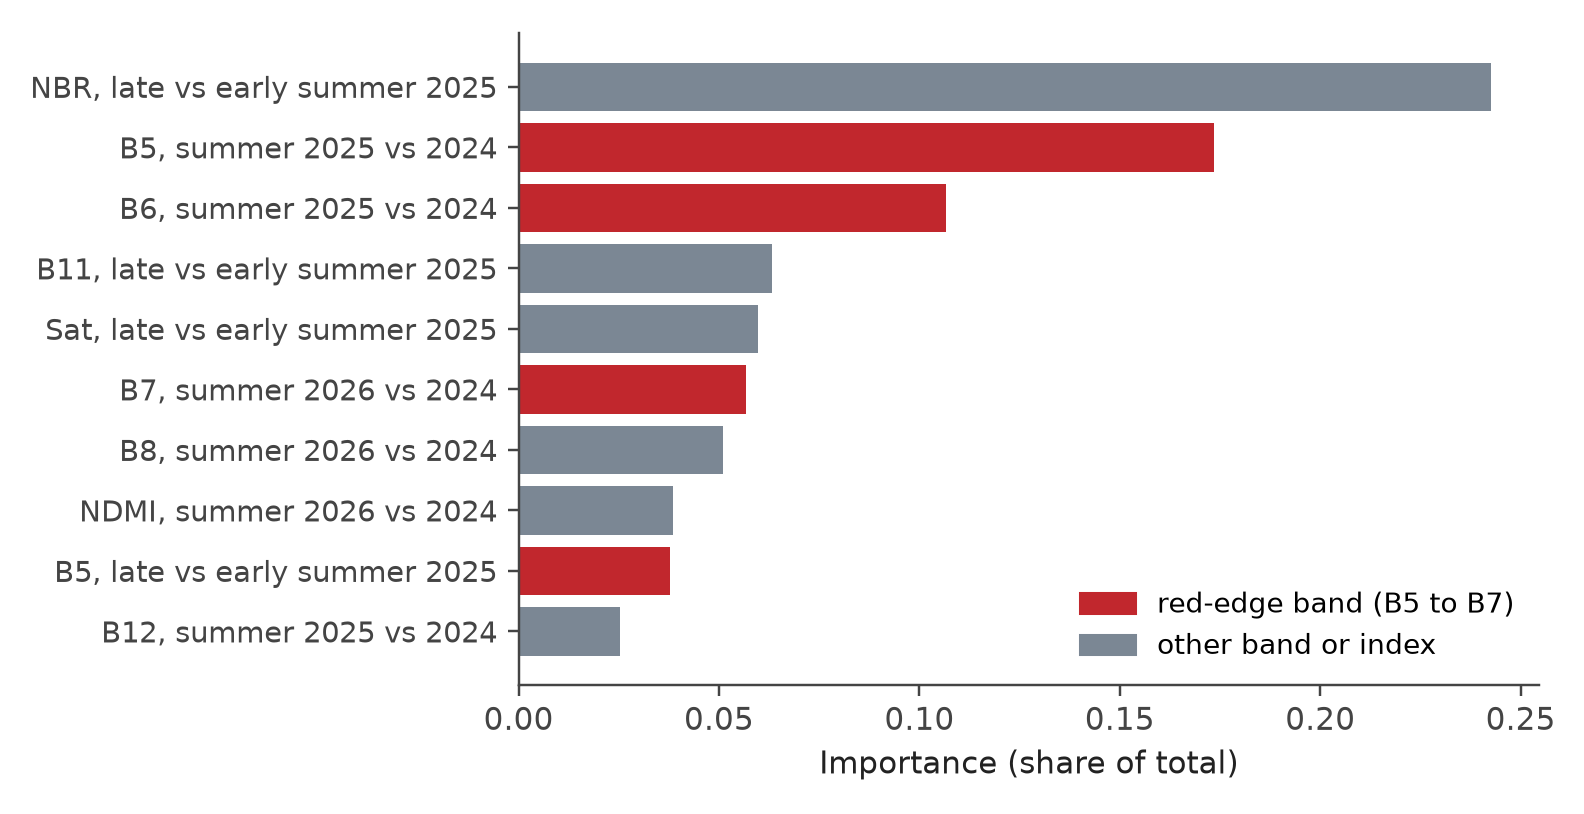
\includegraphics[width=0.78\linewidth]{fig_beetle_importance.png}
\caption{The ten measures gradient boosting relies on most. Each is the change in a band or index between two periods.}\label{fig:importance}
\end{figure}

\begin{itemize}
\item \textbf{It learns what is not damage.} At Moor House, Trout Beck the rule reads 0.55 against a survey score of 0, because the whole bog changed colour over summer 2025. From the undamaged count areas, gradient boosting learned that this kind of greying is not beetle damage and reads 0.05; the final estimate is 0.30.
\item \textbf{The rule keeps the range.} Gradient boosting alone compresses the heavily damaged count areas (Snilesworth, Lodge: rule 0.92, gradient boosting 0.57, survey 0.8). Averaging keeps the strengths of both.
\item \textbf{Red edge matters.} After the change in NBR between early and late summer 2025, the measures the model relies on most are the red-edge bands B5 and B6 between summers 2024 and 2025 (\figref{fig:importance}). Four of the top ten are red-edge. Any future beetle model should include them.
\end{itemize}

\subsection{Imagery where satellite and survey differ}\label{sec:imagery}

\begin{figure}[htbp]
\centering
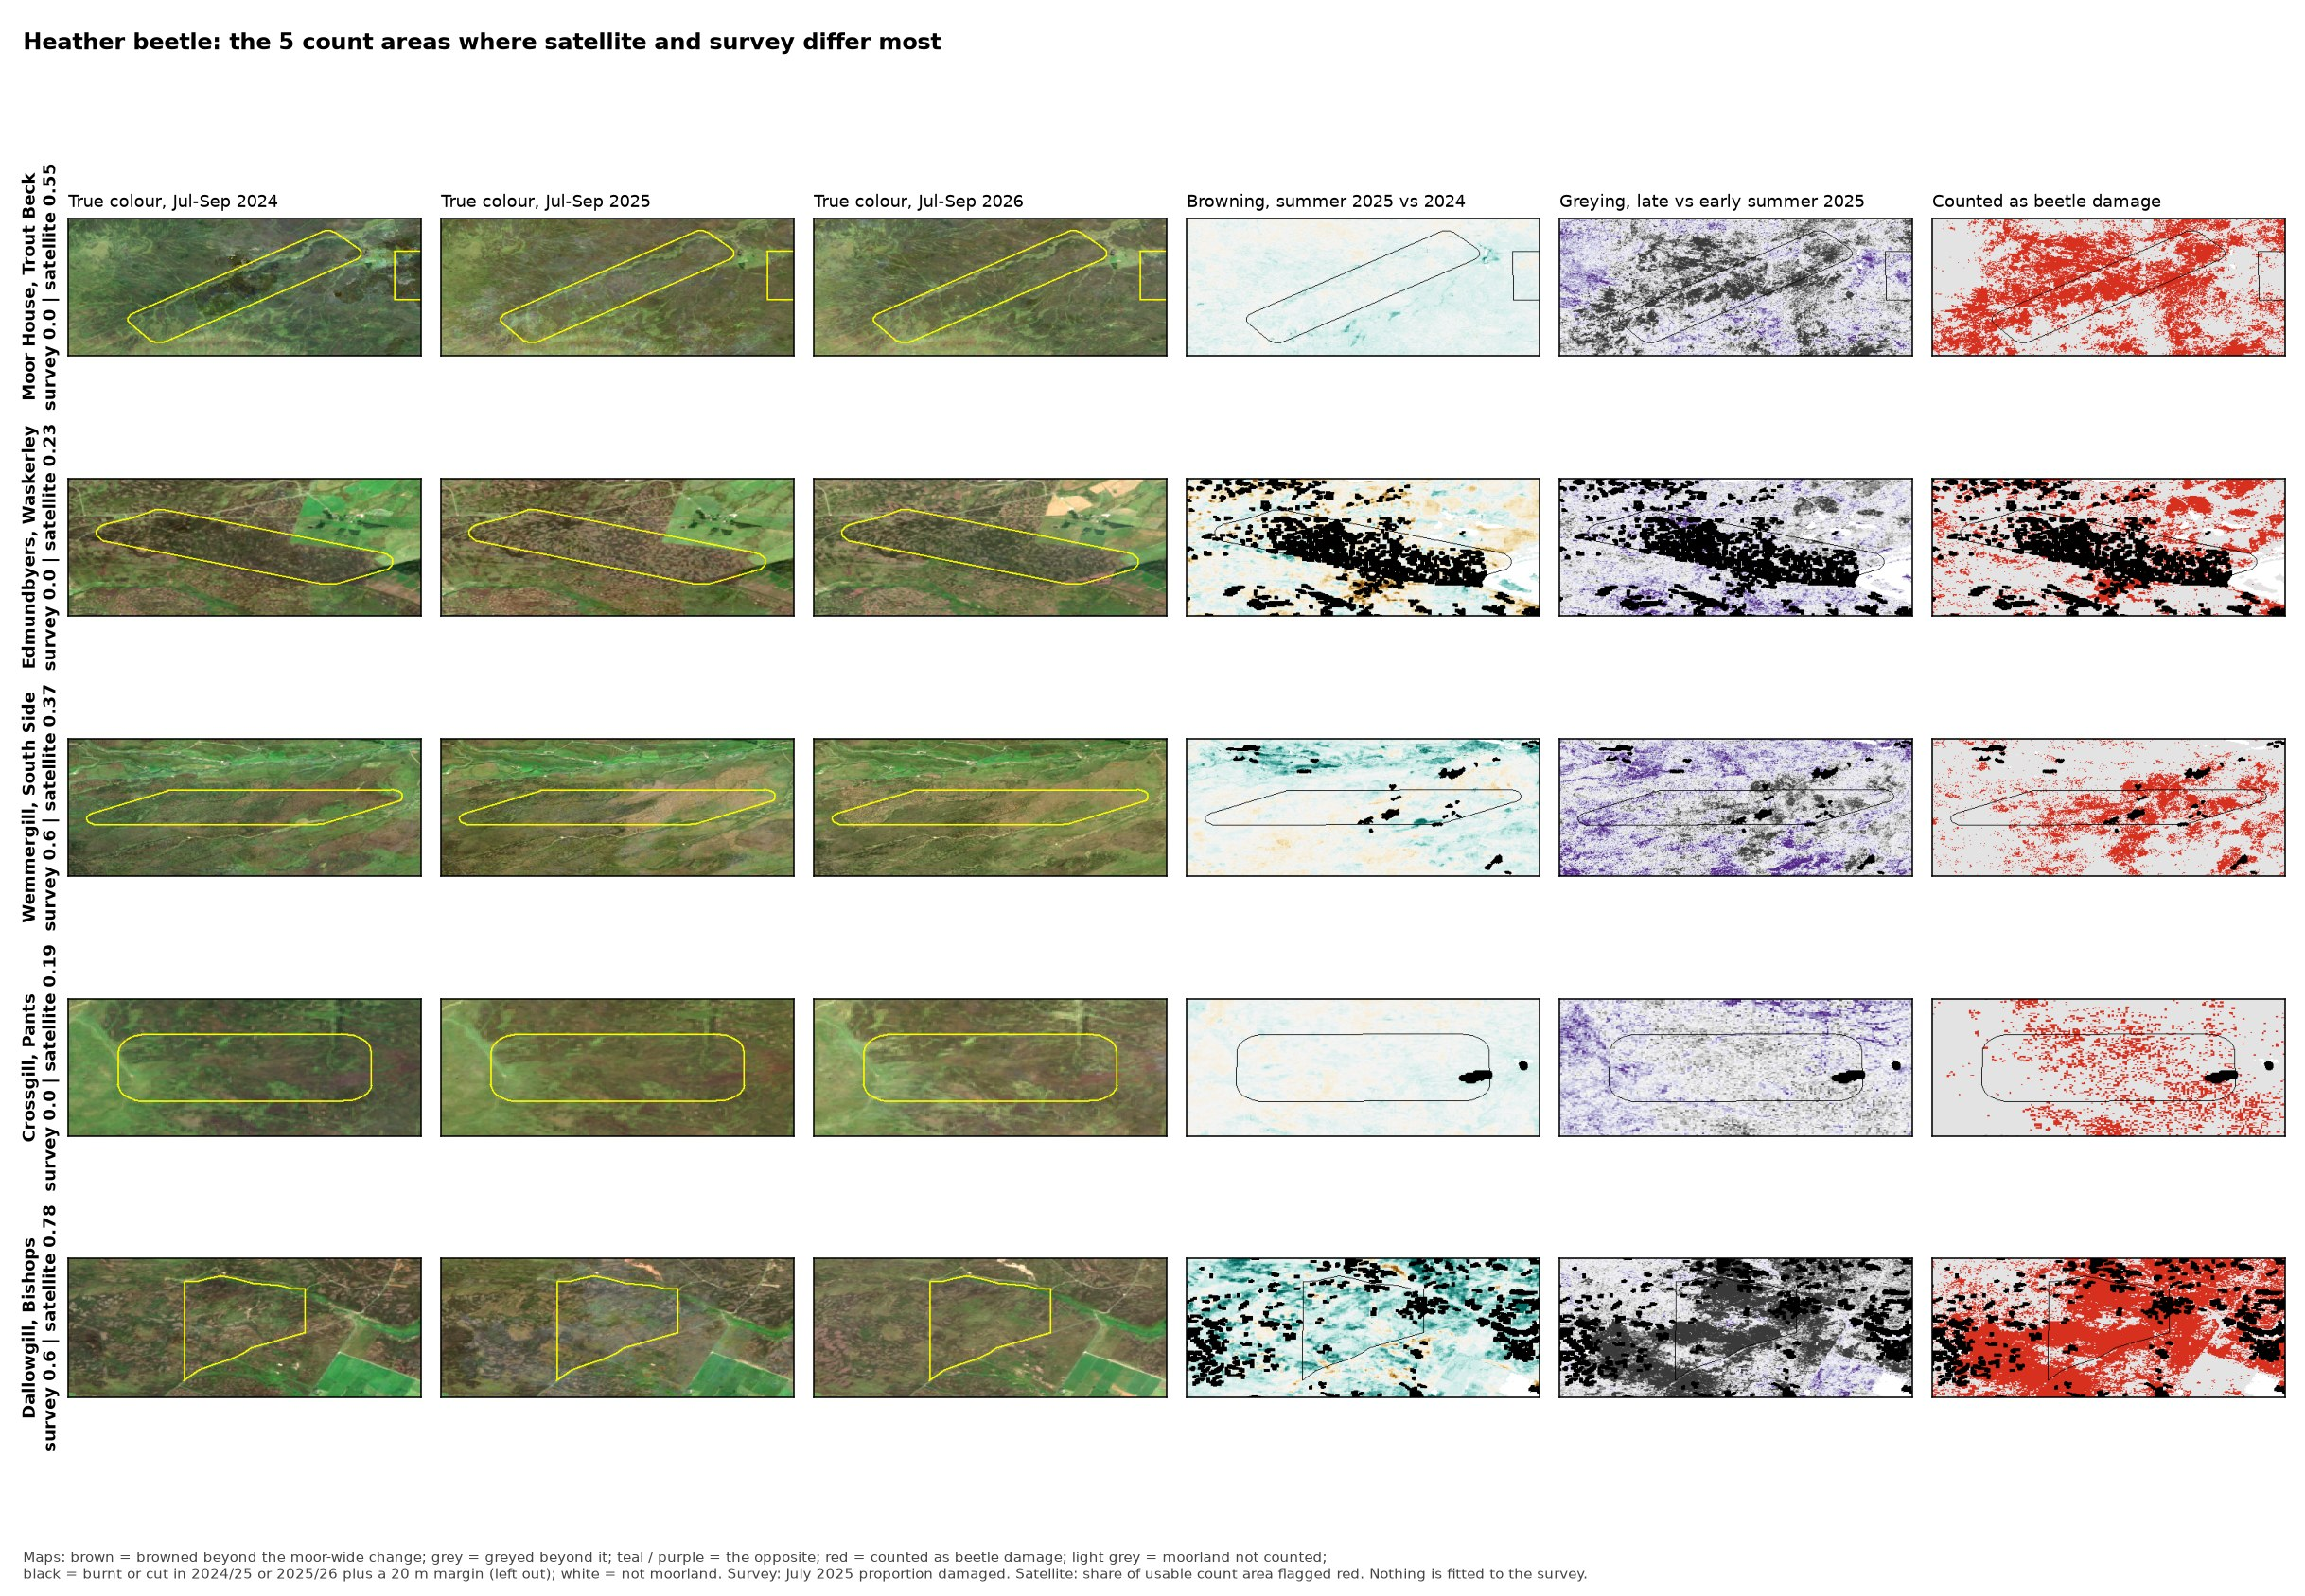
\includegraphics[width=\linewidth]{fig_evidence_disagree.jpg}
\caption{The five count areas where the rule-based estimate and the survey differ most. Left to right: true colour 2024, 2025 and 2026; browning; greying; pixels counted as damage (red). Black is burnt or cut ground plus a 20~m margin.}\label{fig:evidence}
\end{figure}

At 10~m the true-colour images show the damage only faintly; the change maps say more (\figref{fig:evidence}). The same sheet for the five count areas that agree best is in \appref{app:agree}.
\begin{itemize}
\item \textbf{Moor House, Trout Beck} (survey 0, rule 0.55, final 0.30): the greying covers the whole bog, inside and outside the count area. It does not look like beetle damage, and gradient boosting discounts it.
\item \textbf{Edmundbyers, Waskerley} (survey 0, rule 0.23, final 0.20): heavily burnt in 2024/25; the remaining flags sit around the burns, so some burn edges wider than 20~m are still counted.
\item \textbf{Wemmergill, South Side} (survey 0.6, rule 0.37, final 0.24): some flagged patches inside the count area, but fewer than the survey suggests. Field photos would settle it.
\end{itemize}

\subsection{How far the estimate can be trusted}\label{sec:trust}

Leakage means information about the answer reaching the model, which makes results look better than they will be on new data. The design rules out the main routes (\appref{app:leakage}): the model never sees the moor it predicts, the line converting probability to a proportion is fitted on held-out predictions, and every measure is an image change, not a survey score. Three further checks:

\begin{itemize}
\item \textbf{Choosing the model after the fact.} Picking the best of six models on the same 22 count areas flatters the winner. When the model is chosen inside each fold from the training moors only, the final estimate scores 0.105 against 0.098, so the choice adds very little.
\item \textbf{Similar neighbouring moors} (\tabref{tab:region}). When a whole region is hidden from training, gradient boosting alone does markedly worse on it (0.22 against 0.12), because it benefits from having seen similar moors nearby. The final estimate holds up (0.07, close to the rule's 0.08), because the rule needs no training. This is why the final estimate averages the two.
\item \textbf{Chance.} With 22 count areas, differences of 0.01 to 0.02 between methods are within chance: every 90\% bootstrap interval for a model against the rule includes zero (\appref{app:models}). The gain from averaging is consistent across all six models.
\end{itemize}

\begin{table}[htbp]
\centering
\caption{Region hold-out: typical difference on the 8 count areas of the North York Moors and the southern Dales.}\label{tab:region}
\small
\begin{tabular}{lcc}
\toprule
Estimate & Alone & Averaged with the rule \\
\midrule
Rule-based estimate & 0.075 & \\
Gradient boosting, one moor held out & 0.124 & 0.059 \\
Gradient boosting, whole region held out & 0.215 & 0.072 \\
\bottomrule
\end{tabular}
\end{table}

\subsection{Damage and heather management}\label{sec:management}

\begin{table}[htbp]
\centering
\caption{Rank correlation between surveyed damage and the percentage of each count area burnt or cut, by season, and with the change from each count area's usual level (mean of 2017/18 to 2023/24).}\label{tab:management}
\small
\begin{tabular}{lrr}
\toprule
Season & \makecell[r]{Rank correlation with\\\% burnt or cut} & \makecell[r]{Rank correlation with\\change from usual level} \\
\midrule
2023/24 & +0.70 & +0.23 \\
2024/25 & +0.55 & +0.12 \\
2025/26 & +0.33 & $-$0.40 \\
\bottomrule
\end{tabular}

\end{table}

Count areas with more damage were more heavily managed in 2024/25 (rank correlation 0.55; \tabref{tab:management}). They were also the more heavily managed ones before the outbreak (0.70 in 2023/24), and relative to each count area's usual level the 2024/25 increase is spread across count areas. In 2025/26 the most damaged count areas show less management than usual ($-0.40$), possibly because burning or cutting heather that is already dead changes the satellite signal less. Damage scores from 2024 would allow the management response to be traced count area by count area.

The first version of the burning and cutting analysis also reported a ``late'' class: ground that changed only after the burning season. Over half of it fell in summers 2024 and 2025, on count areas the survey scored 0.3 or more, and it followed the survey's damage (rank correlation 0.50). That class was most likely beetle browning, which this report now measures directly.

\FloatBarrier
% ================================================================ 5 discussion
\needspace{12\baselineskip}
\section{Discussion}\label{sec:discussion}

\subsection{What works}

Beetle damage leaves two signals that Sentinel-2 can measure at 10 to 20~m: browning in the summer of the attack and greying as the leaves drop. Measured beyond the change across all count areas, with burnt and cut ground left out, they give a rule-based estimate that already ranks the count areas much as the survey does (0.81) without using the survey at all. Gradient boosting, trained on labels taken from the survey with no hand labelling, adds what the rule cannot do: it learns from undamaged count areas what ordinary seasonal colour change looks like. Averaged, the two give an estimate within 0.1 of the survey on two thirds of the count areas.

The survey scores are themselves estimates in tenths, made by eye over areas of 50 to 290~ha, so agreement much closer than 0.1 cannot be expected. Where the satellite and the survey differ, the imagery suggests reasons on both sides (\secref{sec:imagery}).

\subsection{Limits and how to address them}

\begin{table}[H]
\centering
\caption{Limits and how to address them.}\label{tab:limits}
\footnotesize
\begin{tabularx}{\linewidth}{>{\raggedright\arraybackslash}p{0.25\linewidth}>{\raggedright\arraybackslash}p{0.33\linewidth}L}
\toprule
Limit & Effect & How to address it \\
\midrule
One year, 22 count areas & Small differences between methods are within chance; some choices (greying, averaging) were settled on the same data & A second survey year as a clean test \\
Survey scores by eye, in tenths & Agreement much closer than 0.1 cannot be shown & Field photos with locations; a short note on how scores were made \\
Heather not mapped separately from bog & Bog colour change can read as damage (Trout Beck) & Gradient boosting already discounts it; a few hundred hand-checked patches would help \\
Undamaged ground reads slightly high & About 0.11 above the survey where it found 0 to 0.1 & More undamaged count areas in training \\
Burn edges & Some flags remain round wide burns (Waskerley) & A wider margin where burns are large \\
10~m pixels & Small patches of damage are blurred & PlanetScope (3~m) or aerial imagery \\
\bottomrule
\end{tabularx}
\end{table}

% ================================================================ 6 conclusions
\section{Conclusions and recommendations}\label{sec:conclusions}

Sentinel-2 imagery can measure heather beetle damage on red grouse count areas. A rule-based estimate from browning and greying, averaged with gradient boosting trained on labels taken automatically from the survey, is within 0.1 of the July 2025 survey on 15 of 22 count areas when each moor is predicted without its own data, and it holds up to checks for data leakage. The method can be run on any count area, surveyed or not, at no field cost.

\begin{enumerate}
\item \textbf{Field photos and survey notes.} Photos from the July 2025 survey, ideally with locations, and a short description of how the scores were estimated.
\item \textbf{Damage scores from 2024,} if any exist, to date the outbreak and test the method on a second year.
\item \textbf{Check Neamour, Eggleston} (estimated 0.55, not surveyed), and Wemmergill, South Side and Moor House, Trout Beck, where satellite and survey differ most.
\item \textbf{A second survey year.} Repeating the survey in July 2026 or 2027 on the same count areas would test the method on data it has never seen.
\item \textbf{A few hundred hand-checked patches} (beetle-brown, beetle-grey, burnt, cut, healthy), quickest from Google Earth's historical imagery, would let the model map damage pixel by pixel.
\item \textbf{Keep the red-edge bands} in any future model, and test any new version by holding out one moor at a time.
\item \textbf{PlanetScope} (3~m, near-daily), free under Planet's Education and Research programme, would show smaller patches of damage.
\end{enumerate}

% ================================================================ references
\begin{thebibliography}{99}
\addcontentsline{toc}{section}{References}
\bibitem[Friedman(2001)]{friedman2001} Friedman, J.H. (2001) Greedy function approximation: a gradient boosting machine. \emph{Annals of Statistics}, 29, 1189--1232.
\bibitem[Pedregosa et~al.(2011)]{pedregosa2011} Pedregosa, F., Varoquaux, G., Gramfort, A. et~al. (2011) Scikit-learn: machine learning in Python. \emph{Journal of Machine Learning Research}, 12, 2825--2830.
\bibitem[Roberts et~al.(2017)]{roberts2017} Roberts, D.R., Bahn, V., Ciuti, S. et~al. (2017) Cross-validation strategies for data with temporal, spatial, hierarchical, or phylogenetic structure. \emph{Ecography}, 40, 913--929.
\end{thebibliography}

% ================================================================ appendices
\clearpage
\appendix
\addtocontents{toc}{\protect\vspace{0.6em}{\sffamily\bfseries\color{accent}Appendices}\protect\par\protect\setcounter{tocdepth}{1}}
\renewcommand{\thesection}{\Alph{section}}

\section{Formulae}\label{app:formulae}

Notation: $\rho_k(x)$ is the median surface reflectance of Sentinel-2 band $k$ at pixel $x$ over the clear scenes in a window (digital numbers divided by 10,000). $\mathbf{1}[\cdot]$ is 1 when the condition holds and 0 otherwise.

\subsection{Indices}
\begin{gather*}
\mathrm{NBR} = \frac{\rho_{B8}-\rho_{B12}}{\rho_{B8}+\rho_{B12}}, \qquad \mathrm{NDVI} = \frac{\rho_{B8}-\rho_{B4}}{\rho_{B8}+\rho_{B4}}, \qquad \mathrm{NDMI} = \frac{\rho_{B8}-\rho_{B11}}{\rho_{B8}+\rho_{B11}} \\[4pt]
\text{Brightness} = \tfrac{1}{3}\left(\rho_{B2}+\rho_{B3}+\rho_{B4}\right), \qquad S = \frac{\max(\rho_{B2},\rho_{B3},\rho_{B4})-\min(\rho_{B2},\rho_{B3},\rho_{B4})}{\max(\rho_{B2},\rho_{B3},\rho_{B4})}
\end{gather*}
A scene is clear at $x$ if its s2cloudless cloud probability is below 40\% and its scene classification is not cloud shadow, cloud, cirrus or snow (classes 3, 8, 9, 10, 11).

\subsection{Rule-based estimate}
\begin{gather*}
\Delta\mathrm{NBR}(x) = \mathrm{NBR}_{\text{late 2025}}(x) - \mathrm{NBR}_{\text{2024}}(x), \qquad
\Delta S(x) = S_{\text{late 2025}}(x) - S_{\text{early 2025}}(x)
\end{gather*}
$U$ is the usable ground: moorland, excluding pixels within 20~m of ground detected as burnt or cut in 2024/25 or 2025/26. Each change is centred on its median over $U$ in all count areas (sampled at 20~m):
\[
\Delta\mathrm{NBR}^{*}(x) = \Delta\mathrm{NBR}(x) - \operatorname*{median}_{U}\Delta\mathrm{NBR}, \qquad \Delta S^{*}(x) = \Delta S(x) - \operatorname*{median}_{U}\Delta S
\]
\[
f(x) = \mathbf{1}\!\left[\Delta\mathrm{NBR}^{*}(x) < -0.10 \;\text{ or }\; \Delta S^{*}(x) < -0.05\right], \qquad R_a = \frac{1}{|a\cap U|}\sum_{x\in a\cap U} f(x)
\]

\subsection{Gradient boosting}
\textbf{Labels.} With $d_a$ the surveyed damage of count area $a$, each sampled pixel $x$ in $a$ gets
\[
y_x = \begin{cases}0 & d_a = 0\\ 1 & d_a \ge 0.5\\ \text{no label} & \text{otherwise.}\end{cases}
\]
\textbf{Measures.} $z_x$ holds 45 changes: 15 measures (bands B2, B3, B4, B5, B6, B7, B8, B8A, B11, B12; NBR, NDVI, NDMI, $S$, brightness) for each of three comparisons (summer 2025 minus summer 2024; late minus early summer 2025; summer 2026 minus summer 2024).

\textbf{Model} \citep{friedman2001,pedregosa2011}. An additive score from $M$ regression trees $h_m$ of depth 3:
\[
F_M(z) = F_0 + \nu\sum_{m=1}^{M} h_m(z), \qquad p(z) = \frac{1}{1+e^{-F_M(z)}}
\]
Each tree is fitted, on a random 80\% of the labelled pixels, to the negative gradient of the log-loss
\[
L = -\sum_x \left[\,y_x \log p(z_x) + (1-y_x)\log\!\left(1-p(z_x)\right)\right]
\]
with learning rate $\nu = 0.05$ and $M = 150$ trees.

\textbf{From pixels to a count area.} The mean probability $\bar p_a = \frac{1}{n_a}\sum_{x\in a} p(z_x)$ is mapped to a proportion with a straight line fitted by least squares on the training count areas, using out-of-fold probabilities (five folds split by moor):
\[
\hat d_a = \min\!\left(1,\ \max\!\left(0,\ \alpha + \beta\,\bar p_a\right)\right), \qquad \text{final estimate } \hat c_a = \tfrac{1}{2}\left(R_a + \hat d_a\right)
\]

\subsection{Evaluation}
\textbf{Leave-one-moor-out.} For each moor $m$, the model and its calibration line are fitted using only the other moors' pixels and survey scores; $\hat c_a$ is then computed for the count areas of $m$. The moor-wide medians use imagery from all count areas but no survey scores.
\[
\text{Typical difference} = \frac{1}{n}\sum_{a=1}^{n}\left|\hat c_a - d_a\right|, \qquad \text{Within } k = \#\left\{a : \left|\hat c_a - d_a\right| \le k\right\}
\]
\textbf{Rank agreement} is Spearman's $\rho$: the Pearson correlation of the ranks of $\hat c_a$ and $d_a$.

\textbf{Paired bootstrap.} For $b = 1,\dots,5000$, draw $n$ count areas with replacement and compute the difference in typical difference between a model and the rule on that sample; the 90\% interval is the 5th to 95th percentile.

\textbf{Nested model choice.} For each held-out moor, the training moors are split into five groups; each candidate model is scored by holding out each group in turn, and the best one alone predicts the held-out moor.

\textbf{Region hold-out.} As leave-one-moor-out, but every moor in one GWCT region is held out together (North York Moors; southern Dales). The northern Dales cannot be held out: they contain every count area scored 0.

\textbf{Count areas not surveyed.} The model and calibration line are fitted on all 22 scored count areas and applied to the five unscored ones.

\clearpage
\section{Six models compared}\label{app:models}

\begin{table}[H]
\centering
\caption{Six models for Step 2, alone and averaged with the rule-based estimate. 22 count areas, leave-one-moor-out. The interval is the paired-bootstrap 90\% interval for the change in typical difference against the rule alone; negative is better.}\label{tab:models}
\scriptsize
\setlength{\tabcolsep}{3.5pt}
\begin{tabular}{lrrrrrrrl}
\toprule
& \multicolumn{3}{c}{Model alone} & \multicolumn{5}{c}{Averaged with the rule} \\ \cmidrule(lr){2-4}\cmidrule(lr){5-9}Model & \makecell[r]{Typical\\diff.} & \makecell[r]{Within\\0.1} & \makecell[r]{Rank\\$\rho$} & \makecell[r]{Typical\\diff.} & \makecell[r]{Within\\0.1} & \makecell[r]{Within\\0.2} & \makecell[r]{Rank\\$\rho$} & \makecell[l]{90\% interval\\vs rule} \\
\midrule
Rule-based estimate only & 0.122 & 12 & 0.81 &  &  &  &  &  \\
\midrule
\textbf{Gradient boosting (classic)} & 0.118 & 10 & 0.79 & 0.098 & 15 & 19 & 0.88 & $-$0.053 to $+$0.003 \\
Gradient boosting (LightGBM style) & 0.122 & 10 & 0.78 & 0.101 & 15 & 20 & 0.87 & $-$0.049 to $+$0.006 \\
Support vector machine & 0.124 & 11 & 0.78 & 0.102 & 15 & 20 & 0.86 & $-$0.049 to $+$0.008 \\
Random forest & 0.141 & 12 & 0.78 & 0.109 & 14 & 19 & 0.86 & $-$0.043 to $+$0.013 \\
Logistic regression & 0.151 & 9 & 0.72 & 0.109 & 13 & 19 & 0.84 & $-$0.043 to $+$0.018 \\
Extra trees & 0.161 & 9 & 0.71 & 0.118 & 11 & 19 & 0.83 & $-$0.032 to $+$0.022 \\
\bottomrule
\end{tabular}

\end{table}

All six models improve on the rule when averaged with it, with typical differences of 0.10 to 0.12. Classic gradient boosting is best (0.098) and is used in this report. Settings were fixed in advance: 150 trees of depth 3, learning rate 0.05, 80\% subsampling. More and better labels will matter more than the choice of algorithm.

\section{Earlier attempts}\label{app:early}

\begin{itemize}
\item \textbf{Browning alone} (share of pixels whose NBR fell by more than 0.10, with no moor-wide correction): typical difference 0.27, rank agreement 0.60. The whole area browned in the dry summer of 2025.
\item \textbf{Without the 20~m margin} round burnt and cut ground: typical difference 0.13. Fresh burn edges were counted as damage.
\item \textbf{A heather mask from seasonal greenness} (heather stays green in winter, bog grasses do not): typical difference 0.15, worse than without it. ESA WorldCover labels 98.5\% of the count areas as grassland and none as shrubland, so no ready-made heather map exists for them.
\item \textbf{Calibrating the rule} with a straight line fitted on the other moors: 0.125 against 0.123 uncalibrated, so the rule is used as it stands.
\item \textbf{A random forest on its own:} 0.13 as a classifier of healthy and damaged pixels, and 0.16 predicting each pixel's survey score directly; averaged with the rule it reaches 0.11.
\end{itemize}

\section{Checks for data leakage}\label{app:leakage}

\begin{table}[H]
\centering
\caption{Possible sources of leakage and how they are handled.}\label{tab:leakage}
\footnotesize
\begin{tabularx}{\linewidth}{>{\raggedright\arraybackslash}p{0.36\linewidth}L}
\toprule
Possible leak & How it is handled \\
\midrule
A moor's own pixels or survey score used to predict it & Never: every estimate comes from a model trained without that moor \\
Calibration fitted on the model's own training fit & The line uses out-of-fold probabilities, split by moor \\
Measures built from survey scores & All measures are image changes \\
Settings tuned on the test results & Model settings were fixed in advance \\
Moor-wide reference includes the held-out moor & Imagery only, no survey scores; one moor barely moves a median over 4,000~ha \\
Choosing the best of six models on the same data & Nested test: 0.105 against 0.098; classic gradient boosting chosen in 9 of 15 folds \\
Similar neighbouring moors in training & Region hold-out (\tabref{tab:region}) \\
\bottomrule
\end{tabularx}
\end{table}

\clearpage
\section{Estimates for every count area}\label{app:areas}

\begin{table}[H]
\centering
\caption{Surveyed damage and satellite estimates by count area, each moor predicted without its own data. Grinton, Long Gill (survey 0.5) had too few clear images and is not estimated. The five Eggleston count areas at the foot were not surveyed.}\label{tab:areas}
\footnotesize
\begin{tabular}{lrrrrr}
\toprule
Count area & Survey & Rule & \makecell[r]{Gradient\\boosting} & \makecell[r]{Final\\estimate} & Difference \\
\midrule
\multicolumn{6}{l}{\textit{North York Moors}} \\
Danby, Low Moor & 0.5 & 0.51 & 0.61 & \textbf{0.56} & +0.06 \\
Westerdale, Tank & 0.5 & 0.54 & 0.65 & \textbf{0.59} & +0.09 \\
Rosedale, Pits & 0.6 & 0.69 & 0.66 & \textbf{0.67} & +0.07 \\
Danby, Glaisdale & 0.7 & 0.76 & 0.65 & \textbf{0.70} & +0.00 \\
Snilesworth, Lodge & 0.8 & 0.92 & 0.57 & \textbf{0.74} & $-$0.06 \\
\midrule
\multicolumn{6}{l}{\textit{Southern Dales and Peak}} \\
Ramsgill, Raygill & 0.2 & 0.22 & 0.39 & \textbf{0.30} & +0.10 \\
Dallowgill, Bishops & 0.6 & 0.78 & 0.53 & \textbf{0.66} & +0.06 \\
Swinton, Potts & 0.7 & 0.78 & 0.56 & \textbf{0.67} & $-$0.03 \\
\midrule
\multicolumn{6}{l}{\textit{Northern Dales}} \\
Bollihope, Pikestone Fell & 0.0 & 0.14 & 0.13 & \textbf{0.13} & +0.13 \\
Crossgill, Dowks & 0.0 & 0.02 & 0.17 & \textbf{0.09} & +0.09 \\
Crossgill, Pants & 0.0 & 0.19 & 0.14 & \textbf{0.16} & +0.16 \\
Edmundbyers, Waskerley & 0.0 & 0.23 & 0.17 & \textbf{0.20} & +0.20 \\
Geltsdale, Middle & 0.0 & 0.13 & 0.00 & \textbf{0.07} & +0.07 \\
Moor House, Trout Beck & 0.0 & 0.55 & 0.05 & \textbf{0.30} & +0.30 \\
Moor House, Behind House & 0.0 & 0.10 & 0.01 & \textbf{0.05} & +0.05 \\
Stags Fell, Beacon & 0.0 & 0.08 & 0.00 & \textbf{0.04} & +0.04 \\
Crossgill, Greencastles & 0.1 & 0.03 & 0.24 & \textbf{0.14} & +0.04 \\
Wemmergill, Close House & 0.1 & 0.20 & 0.01 & \textbf{0.11} & +0.01 \\
Bollihope, Catterick & 0.3 & 0.41 & 0.47 & \textbf{0.44} & +0.14 \\
Eggleston, Ever Rigg & 0.3 & 0.31 & 0.29 & \textbf{0.30} & +0.00 \\
Eggleston, Blackton & 0.3 & 0.43 & 0.34 & \textbf{0.38} & +0.08 \\
Wemmergill, South Side & 0.6 & 0.37 & 0.11 & \textbf{0.24} & $-$0.36 \\
\midrule
\multicolumn{6}{l}{\textit{Not surveyed (Northern Dales)}} \\
Eggleston, Neamour &  & 0.70 & 0.39 & \textbf{0.55} &  \\
Eggleston, Cloudlam &  & 0.23 & 0.32 & \textbf{0.27} &  \\
Eggleston, North Sharnberry &  & 0.26 & 0.21 & \textbf{0.23} &  \\
Eggleston, South Sharnberry &  & 0.22 & 0.10 & \textbf{0.16} &  \\
Eggleston, Robin Weathers &  & 0.15 & 0.15 & \textbf{0.15} &  \\
\bottomrule
\end{tabular}

\end{table}

\section{Imagery where satellite and survey agree}\label{app:agree}

\begin{figure}[H]
\centering
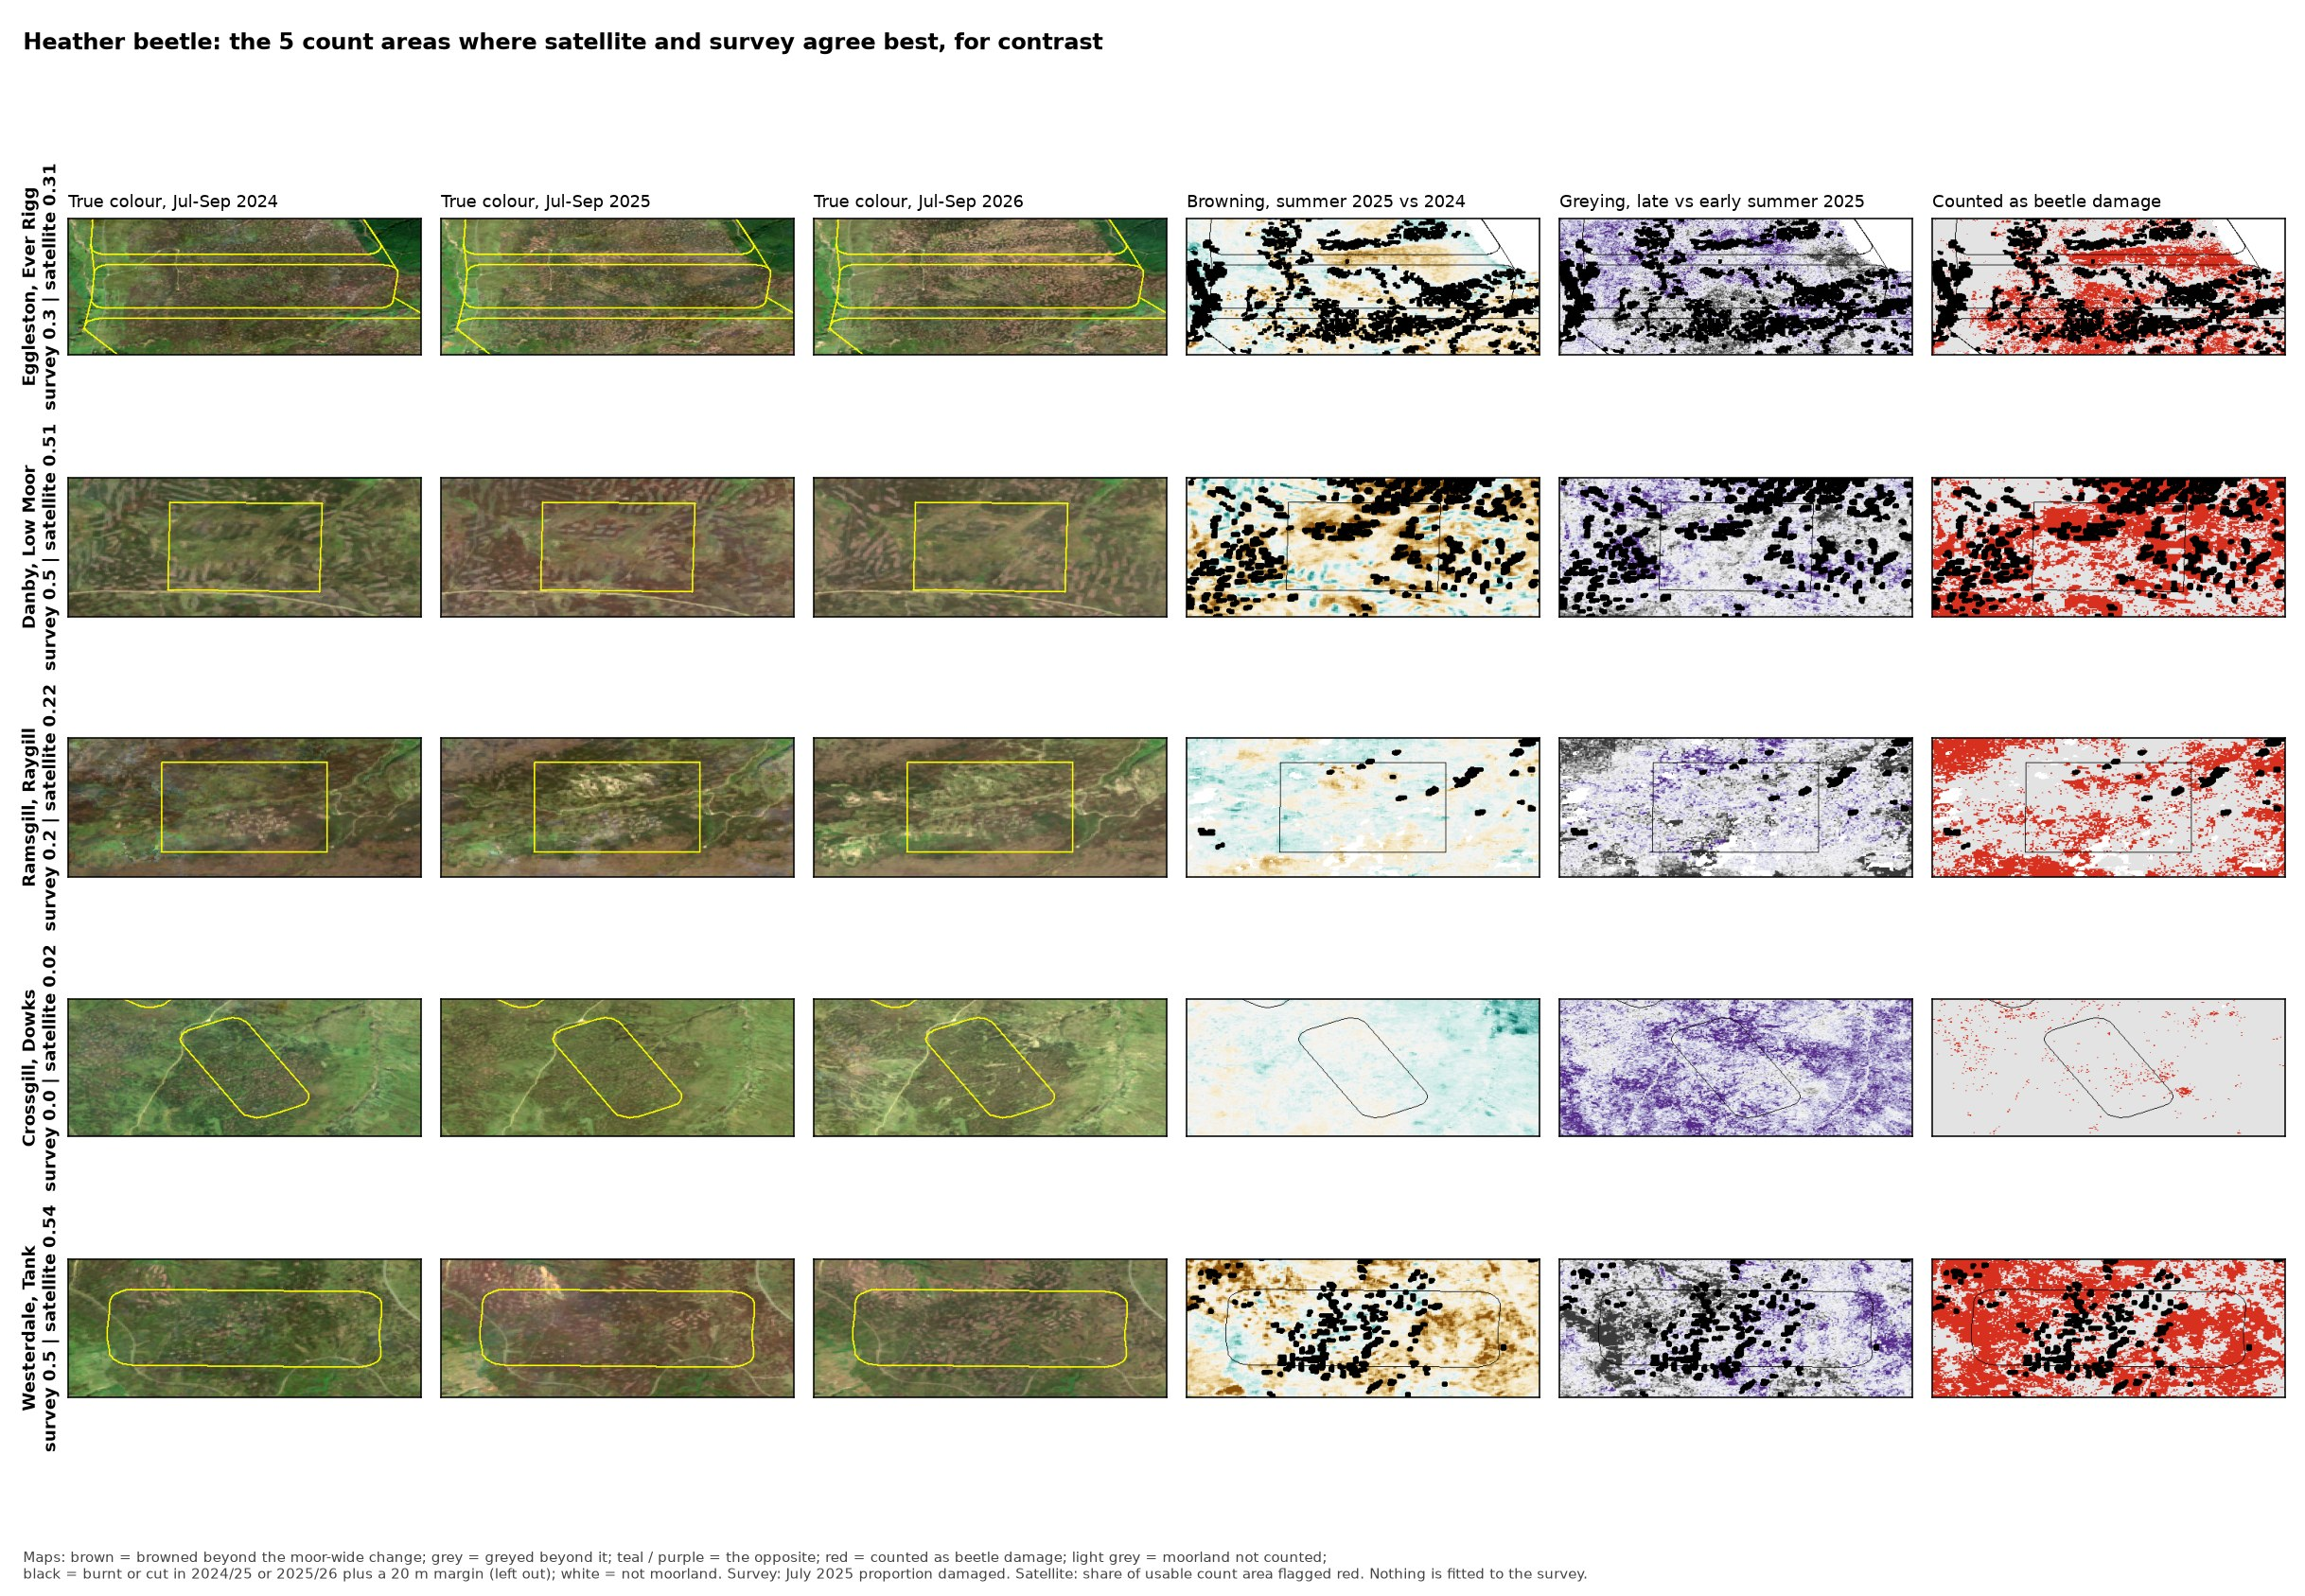
\includegraphics[width=\linewidth]{fig_evidence_agree.jpg}
\caption{The five count areas where the rule-based estimate and the survey agree best. Panels as in \figref{fig:evidence}.}\label{fig:agree}
\end{figure}

\section{Data and code}\label{app:code}

\begin{table}[H]
\centering
\caption{Files behind this report.}\label{tab:files}
\footnotesize
\begin{tabularx}{\linewidth}{>{\raggedright\arraybackslash}p{0.40\linewidth}L}
\toprule
File & Contents \\
\midrule
\texttt{reference/}\newline\texttt{HEATHER\_BEETLE\_DAMAGE\_SUMMER\_2025.xlsx} & The July 2025 survey \\
\texttt{beetle\_check.py} & Image changes per count area; rule-based estimate; comparison with the survey \\
\texttt{beetle\_rf.py} & Samples pixels and their 45 changes (\texttt{rf\_samples.csv}) \\
\texttt{beetle\_model\_compare.py} & Six models, gradient boosting, leakage tests \\
\texttt{beetle\_unscored.py} & Estimates for count areas the survey did not score \\
\texttt{beetle\_evidence.py} & Image sheets \\
\texttt{report/make\_beetle\_figures.py} & Every figure and table in this report, from the outputs \\
\texttt{outputs/beetle\_check/} & All beetle outputs \\
\bottomrule
\end{tabularx}
\end{table}

\end{document}
